\documentclass[12pt,a4paper]{article}

\usepackage[utf8]{inputenc}
\usepackage[T1]{fontenc}
\usepackage[spanish]{babel}
\usepackage{amsmath, amssymb}
\usepackage{graphicx}
\usepackage{float}
\usepackage{geometry}
\geometry{margin=2.5cm}
\usepackage{hyperref}
\usepackage{caption}
\usepackage{subcaption}
\usepackage{setspace}
\usepackage{titlesec}
\usepackage{siunitx}
\usepackage{xcolor} 
    \definecolor{codegreen}{rgb}{0,0.6,0}
    \definecolor{codegray}{rgb}{0.5,0.5,0.5}
    \definecolor{codepurple}{rgb}{0.58,0,0.82}
\usepackage{listings}
\renewcommand{\lstlistingname}{Anexo}


\onehalfspacing

% Para circuitos
\usepackage{circuitikz}

% Datos
\author{Nombre y Apellido \\ Legajo: XXXXX}
\date{\today}

\begin{document}

\setcounter{secnumdepth}{5}
\setcounter{tocdepth}{4}
\titleformat{\paragraph}[block]
  {\normalfont\normalsize\bfseries}
  {\theparagraph}                
  {1em}                            
  {}

      \lstdefinestyle{mystyle}{
    commentstyle=\color{codegreen},
    keywordstyle=\color{magenta},
    numberstyle=\tiny\color{codegray},
    stringstyle=\color{codepurple},
    basicstyle=\scriptsize\ttfamily, 
    breakatwhitespace=false,         
    breaklines=true,                 
    captionpos=b,                    
    keepspaces=true,                 
    numbers=left,                    
    numbersep=5pt,                   
    showspaces=false,                
    showstringspaces=false,
    showtabs=false,                  
    tabsize=2,
    frame=single,                  
    rulecolor=\color{black},
    title=\lstname               
}

\lstset{style=mystyle}

% Carátula personalizada
\begin{titlepage}
    \centering
    
\includegraphics[width=0.25\textwidth]{escudo.png} 
    \hspace{1cm}
    
\includegraphics[width=0.3\textwidth]{download.png} \\[1cm]

    {\large \textbf{UNIVERSIDAD NACIONAL DE CÓRDOBA} \\[0.5cm]}
    {\large \textbf {FACULTAD DE CIENCIAS EXACTAS, FÍSICAS Y NATURALES} \\[1cm]}
    {\Large SÍNTESIS DE REDES ACTIVAS \\[1cm]}

    \rule{\textwidth}{0.5pt} \\[0.5cm]
    {\Large \textbf{Trabajo Práctico N°3} \\[0.3cm]}
    {\Large \textbf{Diseño de Amplificadores con Tecnologías VFA y CFA y Compensación} \\[0.3cm]}
    \rule{\textwidth}{0.5pt} \\[1cm]

\begin{tabular}{l l}
\textbf{Profesor Titular:} & Dr. Ing. Ferreyra Pablo \\
\textbf{Profesor Adjunto:} & Ing. Reale Cesar \\
\\
\textbf{Alumnos:} & Dávila Tomassi, Carlos Valentino \\
 & Mendes Rosa, Agustín \\
 & Monja, Ernesto Joaquín \\
\end{tabular}\\[2cm]

{\centering
Año 2025
\par}

\end{titlepage}

% Índice
\tableofcontents
\newpage

\indent
\section{Motivación}

En este trabajo práctico se aplican de conceptos de compensación para el diseño de amplificadores compuestos que utilizan tecnologías de Amplificador Realimentado por Tensión ($VFA$) y Amplificador Realimentado por Corriente ($CFA$). El objetivo primordial es: 

\begin{itemize}
    \item Diseñar y analizar circuitos amplificadores compuestos $VFA-VFA$ y $VFA-CFA$ para obtener una ganancia global ($A_{vf}=20~dB$) y una respuesta óptima de Máxima Planicidad de Módulo ($M\phi \approx 65^{\circ}$ o $Q_p \approx 0,707$). 
    \item Aplicar técnicas de compensación por adelanto (cero-polo) para mejorar el margen de fase y verificar con la respuesta al escalón.
    \item  Comparar los resultados obtenidos mediante el análisis teórico y la simulación para extraer conclusiones sobre las diferencias encontradas.
\end{itemize}


\begin{figure}[H]
    \centering
    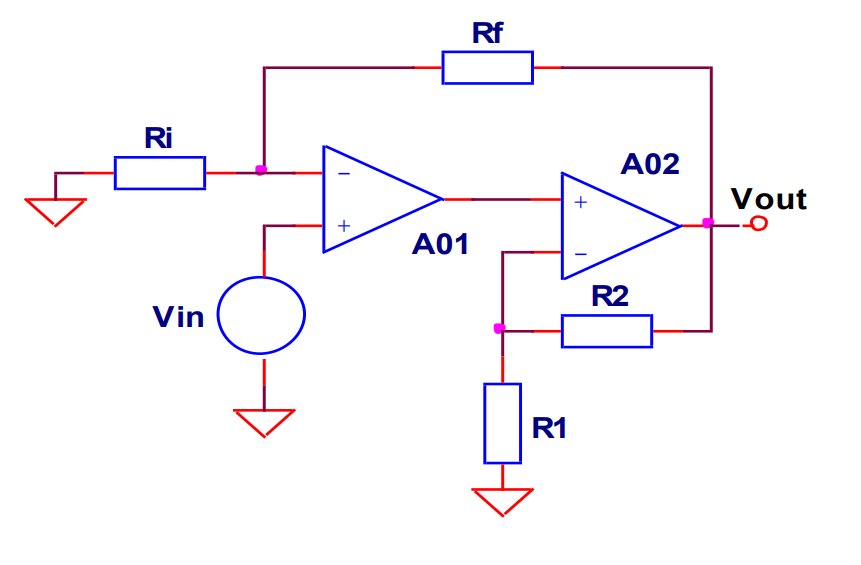
\includegraphics[width=0.75\linewidth]{Consigna.png}
    \caption{Diagrama circuital del amplificador compuesto}
    \label{fig:1}
\end{figure}

\newpage

\section{Marco Teórico}
\subsection{Amplificador Realimentado por Tensión:}
Los Amplificadores Realimentados por Tensión, por sus siglas en inglés, $VFA$ (Voltaje Feedback Amplifier) son un tipo de Amplificador Operacional, cuyo principio de funcionamiento se basa en la detección de un error de tensión entre sus terminales de entrada ($v^+ - v^-$). 

Se caracterizan por tener alta impedancia de entrada y baja impedancia de salida, además de una alta ganancia para modo diferencial y muy alta Relación de Rechazo en Modo Común ($RRMC$). La particularidad de su comportamiento está determinada por la retroalimentación de señales de voltaje, la cual puede lograrse mediante una red de realimentación compuesta por componentes pasivos y/o activos conectados en distintas configuraciones.


\begin{figure}[H]
    \centering
    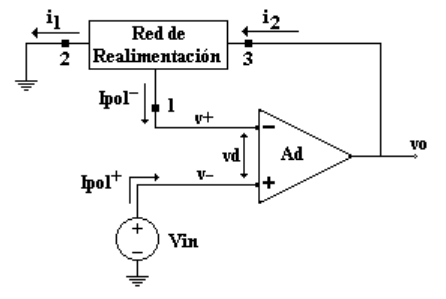
\includegraphics[width=0.5\linewidth]{VFA.png}
    \caption{Diagrama circuital de un $VFA$}
    \label{fig:vfa_diagrama}
\end{figure}

Es posible modelar un Amplificador Operacional según el siguiente circuito:

\begin{figure}[H]
    \centering
    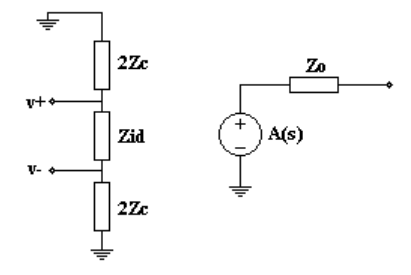
\includegraphics[width=0.5\linewidth]{VFA_modelo.png}
    \caption{Modelo de Amplificador Operacional real}
    \label{fig:placeholder}
\end{figure}

Este modelo real puede simplificarse e idealizarse como se muestra a continuación:

\begin{figure}[H]
    \centering
    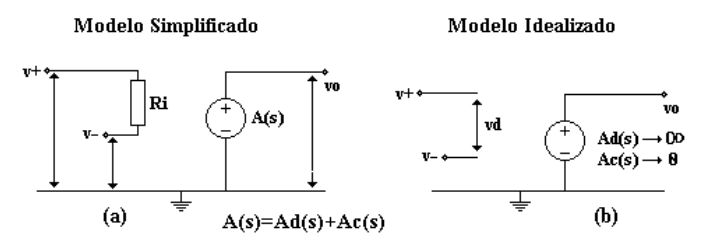
\includegraphics[width=1\linewidth]{VFA_modelo2.png}
        \caption{Modelos alternativos de Amplificador Operacional}
    \label{fig:placeholder}
\end{figure}

Nótese que la salida $v_o$ sólo podrá ser finita si la entrada diferencial $v_d$ es $0$, por lo tanto el amplificador debe ser realimentado de forma negativa (como se ve en la Figura \ref{fig:vfa_diagrama}) para un funcionamiento estable.

Además, si bien se observa que el $VFA$ puede modelarse como una fuente de tensión controlada por tensión, su comportamiento en frecuencia está intrínsecamente limitado por el Producto Ganancia-Ancho de Banda ($GBW = \omega_T$). Debido a que estos dispositivos requieren una compensación por polo dominante interna para garantizar estabilidad, la relación entre la ganancia de lazo cerrado ($A_{vf}$) y la frecuencia de corte ($\omega_c$) se mantiene constante:

\begin{equation}
    \label{eq_1}
    A_{vf} \cdot \omega_c = GBW
\end{equation}
\hspace{0.5 cm}

Este compromiso implica que, al requerir altas ganancias en una etapa, el ancho de banda efectivo se reduce drásticamente, y viceversa. 

En adición a esto, la respuesta dinámica de los $VFA$ también se ve limitada por la corriente finita disponible para cargar el capacitor de compensación interna que se mencionó anteriormente, esta limitación se denomina Slew Rate, y se define como el valor máximo que puede tener la velocidad de crecimiento de la tensión de
salida.
\\

\subsection{Amplificador Realimentado por Corriente:}
Un Amplificador Realimentado por Corriente, por sus siglas en inglés, $CFA$ (Current Feedback Amplifier) es otro tipo de Amplificador Operacional en el cual, a diferencia de un $VFA$, la señal de error es una corriente que circula a través del pin inversor. Su arquitectura se caracteriza por poseer un buffer de tensión interno entre la entrada no inversora ($+$) y la inversora ($-$), lo que otorga a esta última una impedancia de entrada extremadamente baja. 

Además el menor número de internas (en comparación a un $VFA$) resultan en aumento de velocidad, tanto en pequeña como en gran señal, con rangos de operación superiores a $100~[MHz]$ y más de $1000~[V/\mu s]$ de Slew Rate, mostrando producto ganancia ancho de banda del orden del $GHz$, sin embargo con errores en continua mayores que los $VFA$.

Su comportamiento particular de amplificación está principalmente determinado por la retroalimentación de señales de corriente. Por dicho comportamiento también es llamado Amplificador de Transimpedancia, la cual define la tensión de salida por la relación:

\begin{equation}
    \label{eq_2}
V_{out} = I_{in} \cdot Z_T(s)
\end{equation}
\hspace{0.5 cm}

Donde $I_{in}$ es la corriente que se extrae o inyecta en el nodo inversor.

\begin{figure}[H]
    \centering
    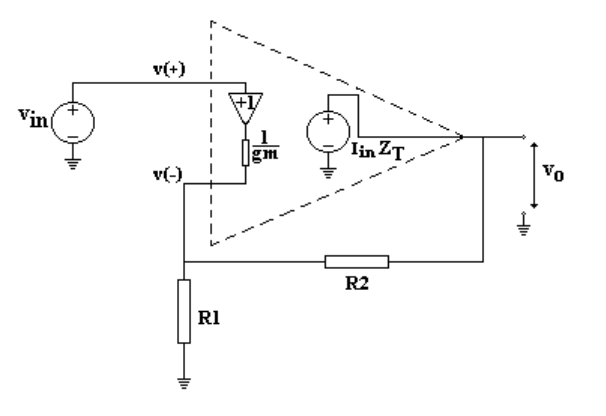
\includegraphics[width=0.75\linewidth]{CFA.png}
    \caption{Diagrama circuital de un CFA}
    \label{fig:cfa_ref}
\end{figure}

Su naturaleza operativa presenta ventajas fundamentales para el diseño de redes activas de alta velocidad, como lo es por ejemplo la independencia del $GBW$ respecto de la ganancia de tensión, ya que el ancho de banda dependerá de la red de realimentación del circuito, además de los altos valores de Slew Rate ya mencionados.

Por lo tanto, puede entenderse que la ganancia y ancho de banda de un amplificador $CFA$ pueden ajustarse mediante las resistencias de la configuración que se ven en la Figura \ref{fig:cfa_ref} (no inversora) de forma independiente, según las siguientes ecuaciones:

\begin{equation}
    \label{eq_3}
    \omega_{CFA} = \frac{1}{C_tR_2}
\end{equation}
\hspace{0.5 cm}

\begin{equation}
    \label{eq_4}
A_{vfi} = 1+\frac{R_2}{R_1}
\end{equation}
\hspace{0.5 cm}

A partir de esto es posible observar que para el diseño de un amplificador con $CFA$, se fija primero el valor de $R_2$ en función del ancho de banda requerido, ya que este es independiente de $R_1$, y después se ajusta el valor de $R_1$ para obtener la ganancia requerida.
\\

\subsection{Compensación y Máxima Planicidad de Módulo:}
Para optimizar la velocidad del sistema, los amplificadores deben operar al límite de su capacidad, para esto es necesario coordinar su estabilidad con los requerimientos de respuesta exigidos. 

El diseño para cubrir estos requerimientos puede suponer el ajuste del comportamiento dinámico del sistema mediante la compensación del amplificador.
\\

\subsubsection{Criterio de Máxima Planicidad de Módulo:}

Éste se utiliza para obtener la respuesta en frecuencia más plana posible en la banda de paso en términos de amplitud, sin picos indeseados. Para llegar a las ecuaciones que describen su comportamiento, se parte de la forma bicuadrática generalizada normalizada respecto a su valor en continua:

\begin{equation}
    \label{eq_5}
    a_{vf}(s) = \frac{A_{vf}(s)}{A_{vf}(0)} = \frac{1 + \frac{s}{\omega_z Q_z} + \frac{s^2}{\omega_z^2}}{1 + \frac{s}{\omega_p Q_p} + \frac{s^2}{\omega_p^2}}
\end{equation}
\hspace{0.5 cm}

Se normaliza (\ref{eq_5}) en frecuencia según $\frac{j\omega}{\omega_p} = j\Omega =S$ :

\begin{equation}
    \label{eq_6}
    a_{vf}(S) = \frac{1 + \frac{S \omega_p }{\omega_z Q_z} + \frac{S^2 \omega_p^2}{\omega_z^2}}{1 + \frac{S}{Q_p} + S^2} = \frac{1 + n_1 S + n_2 S^2}{1 + d_1 S + d_2 S^2}
\end{equation}
\begin{equation}
    \label{eq_7}
    a_{vf}(j\Omega) = \frac{(1 - n_2 \Omega^2) + jn_1 \Omega}{(1 - d_2 \Omega^2) + jd_1 \Omega}
\end{equation}
\hspace{0.5 cm}

Para encontrar Máxima Planicidad de Módulo, se eleva al cuadrado el módulo de la expresión (\ref{eq_7}), tal que:

    \begin{equation}
        \label{eq_8}
        |a_{vf}(j\Omega)|^2 = \frac{(1 - n_2 \Omega^2)^2 + (n_1 \Omega)^2}{(1 - d_2 \Omega^2)^2 + (d_1 \Omega)^2} = \frac{1 + a_1\Omega^2 + a_2\Omega^4}{1 + b_1\Omega^2 + b_2\Omega^4}
    \end{equation}
    \hspace{0.5 cm}


En (\ref{eq_8}), se tiene que se trata de una función par en $\Omega$ y se infiere que la condición de invarianza del módulo respecto a la frecuencia exige a los coeficientes de las potencias homólogas que sean iguales. Por lo que se determina que para:

\[
|a_{vf}(j\Omega)|=cte. \xrightarrow{} a_i = b_i \ \forall \ \Omega \ / \ 0 \leqslant \omega \leqslant \infty
\]
    \hspace{0.5 cm}

    
Nótese que si el grado de $N(s)$ es inferior al de $D(s)$, la condición recién expuesta solo se deberá satisfacer de forma parcial, por lo tanto resulta de interés profundizar el análisis para el caso de que $N(s)$ sea de grado 0 tal que partiendo de (\ref{eq_6}) y aplicando esta condición, resulta que:

    \begin{equation}
        \label{eq_9}
        a_{vf}(S) = \frac{1}{1 + \frac{S}{Q_p} + S^2}
    \end{equation}
    \\
    \begin{equation}
        \label{eq_10}
        |a_{vf}(j\Omega)|^2 = \frac{1}{1 + (\frac{1}{Q_p^2} - 2)\Omega^2 + \Omega^4}
    \end{equation}
\hspace{0.5 cm}

    
    Comparando (\ref{eq_10}) con (\ref{eq_8}), se deduce que: $a_1=a_2=0$, $b_1=\frac{1}{Q_p^2}-2$ y que: $b_2=1$ tal que de estos coeficientes, los únicos capaces de satisfacer la maximización de la planicidad del módulo son: $a_1=b_1$ de modo que: 
    \begin{equation}
        \label{eq_11}
        \frac{1}{Q_p^2}-2=0
    \end{equation}
    \begin{equation}
        \label{eq_12}
        Q_p = \frac{1}{\sqrt{2}} \approx 0,707
    \end{equation}
\hspace{0.5 cm}

Por lo tanto, reemplazando lo obtenido en (\ref{eq_12}) con la expresión encontrada de (\ref{eq_10}) y tomando raíz cuadrada en ambos lados de la ecuación, se tiene que:

     \begin{equation}
         \label{eq_13}
         |a_{vf}(j\Omega)| = \frac{1}{\sqrt{1 + \Omega^4}}
     \end{equation}
     \hspace{0.5 cm}

     
    Tal que si buscamos la frecuencia de corte de $-3~[dB]$, se debe cumplir que (\ref{eq_13}) debe ser igual a:
    
    \begin{equation}
        \label{eq_14}
        \frac{1}{\sqrt{1 + \Omega_H^4}} = \frac{1}{\sqrt{2}}
    \end{equation}
    \hspace{0.5 cm}

    
    Se deduce que para cumplirse la ecuación (\ref{eq_14}), se necesita que: $\Omega_H = 1$ y esto implica por definición de la frecuencia normalizada que: $\omega_H = \omega_p$.

 Para evaluar el Margen de Fase asociado a esta solución y para ello se plantea:
 
    \begin{equation}
        \label{eq_15}
        a_{vf}(S) = \frac{1}{1 - \frac{1}{T(S)}} \approxeq \frac{1}{1 + \frac{S}{Q_p} + S^2}
    \end{equation}
    \hspace{0.5 cm}

    
    De la expresión (\ref{eq_15}) se deduce que la ganancia de lazo es igual a:
    
    \begin{equation}
        \label{eq_16}
        T(S) = -\frac{1}{\frac{S}{Q_p} + S^2} = -\frac{1}{S(S + \frac{1}{Q_p})}
    \end{equation}
    \hspace{0.5 cm}

    
    Se determina entonces la frecuencia del punto crítico a partir de la condición de módulo para la estabilidad de un amplificador operacional, siendo esta: $|T(j\Omega_G)|=1$ tal que aplicando esta condición  a la ecuación (\ref{eq_16}), se tiene que:

    \begin{equation}
        \label{eq_17}
        \Omega_G^4 + \frac{1}{Q_p^2} \Omega_G^2 = 1
    \end{equation}
    \hspace{0.5 cm}

    
    Si definimos que: $x=(\Omega_G)^2$ y aplicando lo deducido en (\ref{eq_12}), el sistema se simplifica a una ecuación cuadrática igual a:\\
    
    \begin{equation}
        \label{eq_18}
        x^2 + 2x - 1 = 0
    \end{equation}
    \hspace{0.5 cm}

    
    Donde la solución no negativa es $x_1=0,4142$ y por lo tanto $\Omega_G=\sqrt{x}=\sqrt{0,4142}=0,644$, y $\omega_G = \Omega_G \ \omega_p = 0,644 \ \omega_p$. Finalmente el Margen de Fase para esta condición es:
    
    \begin{equation}
        \label{eq_19}
        M\phi = \ang{180} + \arg(T(j\Omega_G))
    \end{equation}

    \begin{equation}
        \label{eq_20}
        M\phi = \ang{180} - \ang{90} - \arctan(\Omega_G Q_p)  
    \end{equation}
    
    \begin{equation}
        \label{eq_21}
        M\phi = \ang {90} - \arctan\left(\frac{0,644}{\sqrt{2}}\right) 
    \end{equation}
    \hspace{0.5 cm}

    
    Se deduce finalmente de (\ref{eq_21}) que: $M\phi \approx \ang{65,5}$.\\
    \hspace{1 cm}

\subsubsection{Compensación por Adelanto (Red Cero-Polo):}

Se caracteriza por generar el cero a frecuencia igual o superior que el polo original del sistema, anulando el atraso de fase, mientras que el polo generado se encuentra fuera de la banda de utilización. Ésta compensación puede lograrse insertando una red pasiva RC de forma Paralelo-Serie a la salida del amplificador, como la que se ve a continuación:

\begin{figure}[H]
    \centering
    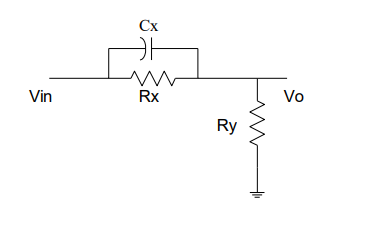
\includegraphics[width=0.5\linewidth]{RC.png}
    \caption{Red RC para Cero-Polo}
    \label{fig:placeholder}
\end{figure}

Ésta red presenta la siguiente función de transferencia:

    \begin{equation}
        \label{eq_22}
        A_C(s) = \frac{A_C(0)\left(1+\frac{s}{\omega_{zc}}\right)}{\left(1+\frac{s}{\omega_{pc}}\right)}
    \end{equation}
    \hspace{0.5 cm}

Y se pueden obtener las variables según la conexión de los componentes, deduciendo entonces:

\begin{equation}
   \label{eq_23}
   A_C(0) = \frac{R_y}{R_y+R_x}
\end{equation}

\begin{equation}
   \label{eq_24}
   \omega_{zc} = \frac{1}{C_xR_x}
\end{equation}

\begin{equation}
   \label{eq_25}
   \omega_{pc} = \frac{1}{C_x(R_x//R_y)}
\end{equation}
\hspace{0.5 cm}

Tal que la función de transferencia puede expresarse como:

   \begin{equation}
        \label{eq_26}
A_C(s) = \left(\frac{R_y}{R_y+R_x}\right)\left(\frac{1+sC_xR_x}{1+sC_x(R_x//R_y)}\right)
    \end{equation}
    \hspace{0.5 cm}

\newpage

\section{Circuito I: VFA-VFA}

\subsection{Objetivo del Circuito I:}

El objetivo de este circuito es evaluar si es posible cumplir simultáneamente con una ganancia global $A_{vf}(s) = 20~[dB]$ y un Margen de Fase $M\phi = \ang{65,5}$, utilizando exclusivamente dos amplificadores $VFA$ y ajustando únicamente las resistencias del lazo de realimentación local.
\\

\subsection{Modelo adoptado:}

Para el análisis de este amplificador compuesto, se pide utilizar un LM324 como VFA, con las siguientes especificaciones:

\begin{itemize}
    \item $A_d(0) = 100~[dB]$
    \item $f_T = 1~[MHz]$
    \item $f_{p1} = 10~[Hz]$        
    \item $f_{p2} = 5,06~[MHz]$
\end{itemize}
\hspace{0.5 cm}

\subsection{Análisis teórico:}

Se hará un breve análisis del circuito sólo con $AO1$, para así evaluar el comportamiento que se deberá imponer luego en el segundo amplificador para llegar a cumplir los requerimientos.

Con un sólo amplificador, la red de realimentación se compone de $R_f$ y $R_i$, por lo que se hace uso de la fórmula de Black para encontrar las expresiones de ganancia necesarias para el análisis:

   \begin{equation}
        \label{eq_27}
A_v(s) = \frac{A_d(0)}{\left(1+\frac{s}{\omega_{p1}}\right)\left(1+\frac{s}{\omega_{p2}}\right)}~~~\xrightarrow{} ~~~GLA~del~VFA
    \end{equation}

   \begin{equation}
        \label{eq_28}
T(s) = \left[\frac{V_{out}}{V_o~'}\right]_{V_{in}=0} = -\frac{A_d(0)\left(\frac{R_i}{R_f+R_i}\right)}{\left(1+\frac{s}{\omega_{p1}}\right)\left(1+\frac{s}{\omega_{p2}}\right)}~~~\xrightarrow{} ~~~GL~del~sistema~simple
    \end{equation}

   \begin{equation}
        \label{eq_29}
A_{vf}(0) = \frac{A_v(0)}{1-T(0)} = \frac{A_d(0)}{1+A_d(0)\left(\frac{R_i}{R_f+R_i}\right)}~~~\xrightarrow{} ~~~GLC~del~sistema~simple
    \end{equation}

   \begin{equation}
        \label{eq_30}
A_{vfi} \approx \frac{R_f + R_i}{R_i} = \left(1 + \frac{R_f}{R_i}\right)~~~\xrightarrow{} ~~~GLC~ideal~del~sistema~simple
    \end{equation}
    \hspace{0.5 cm}


Para cumplir con el requerimiento de ganancia que plantea el objetivo, se define lo siguiente:

   \begin{equation}
        \label{eq_31}
A_{vfi} \approx \left(1 + \frac{R_f}{R_i}\right) = 20~[dB] = 10~[veces]
    \end{equation}

       \begin{equation}
        \label{eq_32}
\frac{R_f}{R_i} = 9 
    \end{equation}
    \hspace{0.5 cm}


A partir de esto se eligen los siguientes valores de resistencias, los cuales suponen un equilibro entre un alto error por tensión de offset (si fuesen valores muy elevados) y la potencia que consumiría el circuito (si fuesen valores muy bajos):

   \begin{equation}
        \label{eq_33}
R_f = 90~[k\Omega]
    \end{equation}

       \begin{equation}
        \label{eq_34}
R_i = 10~[k\Omega] 
    \end{equation}
    \hspace{0.5 cm}

De esta forma puede escribirse la ganancia a lazo cerrado como:

   \begin{equation}
        \label{eq_35}
A_{vf}(s) = \frac{A_v(s)}{1-T(s)} = \frac{\frac{A_d(0)}{\left(1+\frac{s}{\omega_{p1}}\right)\left(1+\frac{s}{\omega_{p2}}\right)}}{1+\frac{A_d(0)}{\left(1+\frac{s}{\omega_{p1}}\right)\left(1+\frac{s}{\omega_{p2}}\right)}\left(\frac{R_i}{R_f+R_i}\right)} \approx  \frac{\left(1 + \frac{R_f}{R_i}\right)}{\left(1+\frac{s}{\omega_{p3}}\right)\left(1+\frac{s}{\omega_{p4}}\right)}
    \end{equation}
    \hspace{0.5 cm}


Para averiguar el valor estos polos se hizo uso de un código de Python que se encuentra en el Anexo (\ref{codigo1}), del cual se obtuvo que:

       \begin{equation}
        \label{eq_36}
f_{p3} = 102~[k\Omega]
\end{equation}

       \begin{equation}
        \label{eq_37}
f_{p4} = 4.9~[M\Omega]
\end{equation}
\hspace{0.5 cm}

Con la ayuda de un código de Python que se encuentra en el Anexo (\ref{codigo2}), se logró graficar la función de transferencia del sistema simple $A_{vf}(s)$ que plantea la ecuación (\ref{eq_35}):

\begin{figure}[H]
    \centering
    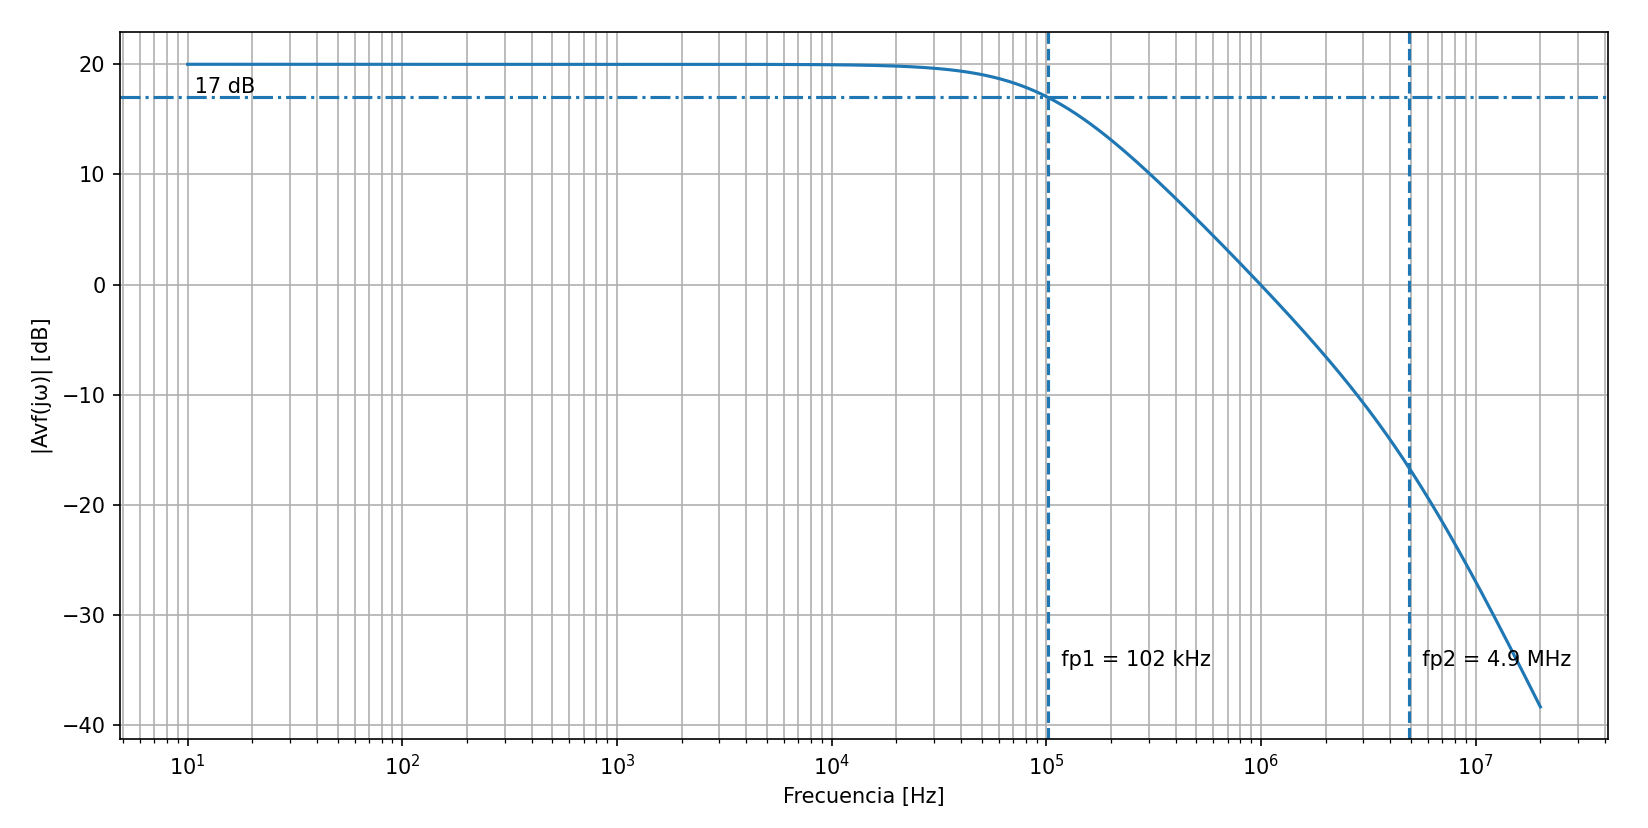
\includegraphics[width=0.9\linewidth]{Avf_simple.png}
    \caption{Respuesta en frecuencia del sistema simple $A_{vf}(s)$}
    \label{fig:placeholder}
\end{figure}

Por la distancia entre los polos, puede determinarse que la frecuencia de corte del sistema está localizado en el primer polo, es decir:

\begin{equation}
        \label{eq_38}
f_H = f_{p3} = 102~[kHz]
\end{equation}
\hspace{0.5 cm}

Analizando la constante $GBW$ a lazo abierto, es posible encontrar la frecuencia del punto crítico actual $(f_G)$, según:

\begin{equation}
        \label{eq_39}
A_v(jf_G).(f_G) = A_v(jf_{p1}).(f_{p1})
\end{equation}

   \begin{equation}
        \label{eq_40}
A_{vfi}.(f_G) = A_d(0).(f_{p1})
    \end{equation}
    \hspace{0.5 cm}

Despejando $f_G$ de la ecuación (\ref{eq_40}) se obtiene:

   \begin{equation}
        \label{eq_41}
f_G = \frac{10^5~[veces]~.~10~[Hz]}{10~[veces]} = 10^5~[Hz] = 100~[kHz]    \end{equation}
    \hspace{0.5 cm}



Luego es posible obtener la frecuencia del punto crítico necesaria $(f_G')$ para alcanzar el Margen de Fase que asegura la condición de Máxima Planicidad de Módulo, partiendo de la expresión de módulo de $T(j\omega)$:

   \begin{equation}
        \label{eq_42}
\left|T(j\omega)\right| = \frac{-A_d(0)\left(\frac{R_i}{R_f+R_i}\right)}{\sqrt{1+\left(\frac{f}{f_{p1}}\right)^2}\sqrt{1+\left(\frac{f}{f_{p2}}\right)^2}}    \end{equation}
    \hspace{0.5 cm}

Tal que entonces tomando las componentes de fase de la ecuación (\ref{eq_42}), el Margen de Fase puede escribirse de la siguiente manera:

   \begin{equation}
        \label{eq_43}
M\phi = \ang{180} - \arctan\left(\frac{f_G'}{f_{p1}}\right) - \arctan\left(\frac{f_G'}{f_{p2}}\right) = \ang{65,5}
\end{equation}

   \begin{equation}
        \label{eq_44}
M\phi = \ang{180} - \ang{90} - \arctan\left(\frac{f_G'}{f_{p2}}\right) = \ang{65,5}
\end{equation}
    \hspace{0.5 cm}

Despejando la frecuencia del punto crítico necesaria $f_G'$, resulta:

  \begin{equation}
        \label{eq_45}
f_G' = f_{p2}.\tan(\ang{180} - \ang{90} - \ang{65,5}) = 5,06 ~[MHz] \cdot 0,4557 \approx 2,306~[MHz]
\end{equation}
    \hspace{0.5 cm}

Comparando los valores se deduce que las compensaciones a realizar deben aumentar el ancho de banda del sistema (dado que $f_G' > f_G$), o modificar la fase de $T(s)$ para que a una misma frecuencia, se mueva el Margen de Fase.\\

Ahora comienza el análisis del amplificador compuesto:

\begin{figure}[H]
    \centering
    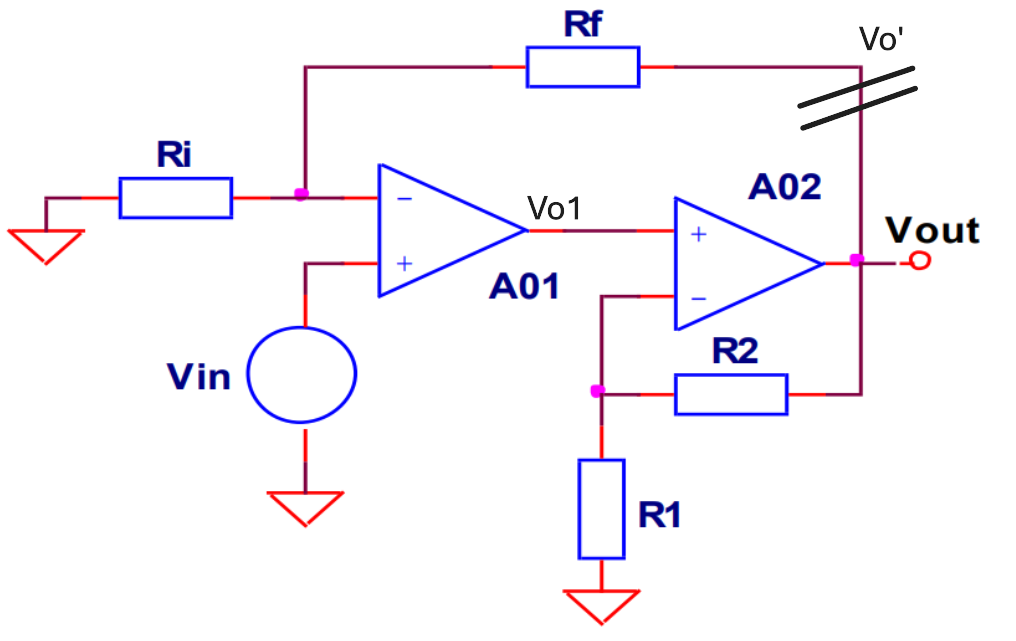
\includegraphics[width=0.6\linewidth]{Teórico_VFAVFA.png}
    \caption{Circuito I. $VFA-VFA$}
    \label{fig:placeholder}
\end{figure}

Se procede a analizar el efecto de $AO2$ sobre las ganancias y el Margen de Fase del sistema, e intentar compensar correctamente para cumplir con el objetivo del circuito I.

Para ello, se modelan ambos amplificadores con la misma función de transferencia a lazo abierto, de acuerdo con los parámetros especificados para el LM324:

   \begin{equation}
        \label{eq_46}
A_{v1}(s) = A_{v2}(s) = A_v(s) = \frac{A_d(0)}{\left(1+\frac{s}{\omega_{p1}}\right)\left(1+\frac{s}{\omega_{p2}}\right)}
\end{equation}
    \hspace{0.5 cm}

El lazo de realimentación local del segundo $VFA$ viene dado por la relación de resistencias $R_1$ y $R_2$, tal que la ganancia de lazo de $AO2$ resulta:

   \begin{equation}
        \label{eq_47}
T_2(s) = -A_v(s)\frac{R_1}{R_1 + R_2}
\end{equation}
    \hspace{0.5 cm}

Y así la ganancia a lazo cerrado de $AO2$ puede escribirse:
    
   \begin{equation}
        \label{eq_48}
A_{vf2}(s) = \frac{A_v(s)}{1-T_2(s)}
\end{equation}
    \hspace{0.5 cm}

Al abrir el lazo de realimentación principal, se encuentra $AO1$ a lazo abierto, y $AO2$ realimentado localmente, por lo que la ganancia de lazo del sistema compuesto es:

   \begin{equation}
        \label{eq_49}
T(s) = -A_{v1}(s)\,A_{vf2}(s)\,\left(\frac{R_i}{R_i + R_f}\right)
\end{equation}
    \hspace{0.5 cm}

Y la ganancia a lazo cerrado total del amplificador compuesto será:

   \begin{equation}
        \label{eq_50}
A_{vf}(s) = \frac{A_{v1}(s)\,A_{vf2}(s)}{1-\left(-A_{v1}(s)\,A_{vf2}(s)\,\left(\frac{R_i}{R_i + R_f}\right)\right)}
\end{equation}
    \hspace{0.5 cm}


A diferencia del caso de un único $VFA$, donde $T(s)$ es de segundo orden, aquí la expresión completa de $T(s)$ resulta de cuarto orden, ya que combina los dos polos de $A_{v1}(s)$ con los polos de $A_{vf2}(s)$, los cuales a su vez dependen explícitamente de la relación entre $R_2$ y $R_1$. En forma general, el denominador de $T(s)$ puede escribirse como:

   \begin{equation}
        \label{eq_51}
D_T(s) = s^4 + a_1\,s^3 + a_2\,s^2 + a_3\,s + a_4
\end{equation}
    \hspace{0.5 cm}

Donde los coeficientes $a_i$ son funciones de $R_1$ y $R_2$ que desplazan a los polos de $T(s)$.
\\

\subsection{Estrategia de diseño:}

El diseño buscado implicaría encontrar una relación entre $(R_1,R_2)$ tal que se cumpla el objetivo del circuito I.
\\

\subsubsection{Modelo Idealizado:}

En un primer intento, si se desprecia el efecto dinámico de $AO2$ y se lo modela únicamente como una ganancia estática (es decir, $A_{vf2}=1+\frac{R_2}{R_1}$), es posible obtener una relación $\tfrac{R_2}{R_1}$ que lleva a un Margen de Fase cercano al requerido.

Con la constante $(GBW=\omega_T)$ se puede obtener la ganancia a lazo abierto del sistema compuesto necesaria para asegurar el Margen de Fase deseado en $f_G$ a partir de lo obtenido en la ecuación (\ref{eq_45}):

   \begin{equation}
        \label{eq_52}
A_v(jf_G)f_G = f_T
\end{equation}

   \begin{equation}
        \label{eq_53}
A_v(jf_G) = \frac{f_T}{f_G} = \frac{1~[MHz]}{2,306~[MHz]} = 0,43367~[veces]= -7,2568~[dB]
\end{equation}
    \hspace{0.5 cm}

La atenuación tiene sentido ya que la frecuencia de punto crítico necesaria para cumplir los requisitos (ecuación (\ref{eq_45})) resultó mayor a la analizada con un solo amplificador, por lo que para llegar al objetivo se debe reducir la ganancia y así aumentar su ancho de banda.

Como la ganancia de lazo debe ser igual a uno en el punto crítico, se escribe:

   \begin{equation}
        \label{eq_54}
\left|T(jf_G)\right| = \left|A_v(jf_G)\right|\left(\frac{R_i}{R_f+R_i}\right)\left(1+\frac{R_2}{R_1}\right) = 1
\end{equation}

   \begin{equation}
        \label{eq_55}
\left|T(jf_G)\right| = 0,43367\left(\frac{1}{10}\right)\left(1+\frac{R_2}{R_1}\right) = 1
\end{equation}
\hspace{0.5 cm}

Por lo que despejando la relación entre $R_2$ y $R_1$, se obtiene:

   \begin{equation}
        \label{eq_56}
\frac{R_2}{R_1} = \frac{10}{0,43367} - 1 = 22,059
\end{equation}
\hspace{0.5 cm}

En base a este resultado obtenido, pueden elegirse:

   \begin{equation}
        \label{eq_57}
R_1 = 1~[k\Omega] ~~~~~~~~~~~~~~R_2 = 22~[k\Omega]
\end{equation}
\hspace{0.5 cm}

Si bien se llega a un resultado que parece correcto, se recuerda que idealizar el comportamiento del segundo amplificador no respeta la dinámica real del sistema. 
\\

\subsubsection{Modelo Real:}

Para tener en cuenta correctamente el efecto de $AO2$, se utilizó el modelo completo $A_{vf2}(s)$ en la expresión de $T(s)$ y se evaluó el lazo mediante barridos de frecuencia utilizando un código de Python incluido en el Anexo (\ref{codigo3}), el cual recorre distintos valores de $\frac{R_2}{R_1}>0$. En los casos analizados se observó que el cruce de ganancia de lazo $|T|=1$ se produce con un Margen de Fase significativamente distinto de $\ang{65,5}$.

\begin{figure}[H]
    \centering
    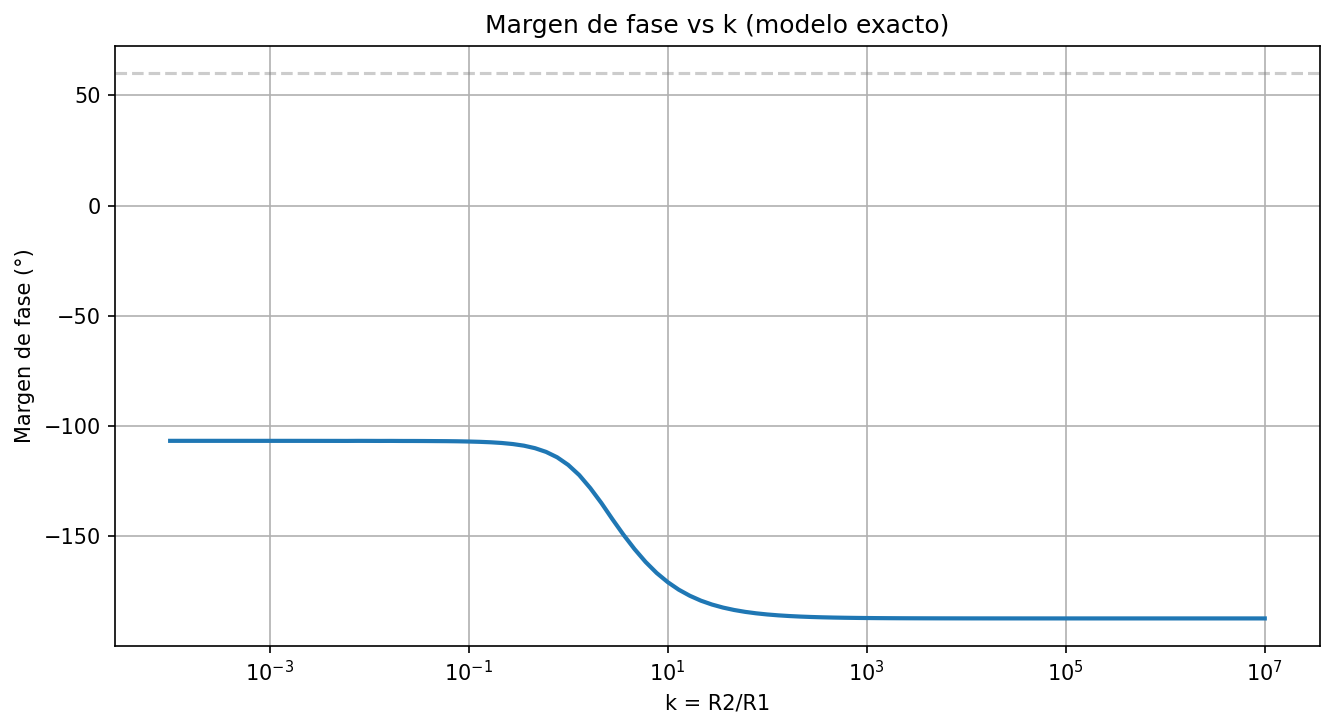
\includegraphics[width=1\linewidth]{k_vs_MF.png}
    \caption{Margen de Fase en función de la relación $R_2/R_1$}
    \label{fig:placeholder}
\end{figure}

Luego se utilizó la iteración manual y un código de Python incluido en el Anexo (\ref{codigo4}) para darle valores negativos a la relación $\frac{R_2}{R_1}$ (debido a que el anterior no admite valores de $\frac{R_2}{R_1}<0$ por ser argumento de una función logarítmica para graficar) y graficar $T(s)$ y $A_{vf}(s)$. En base a esto se obtiene como solución una resistencia efectiva \emph{negativa} para los valores de interés de $T(s)$. El valor que se encuentra como solución es:

   \begin{equation}
        \label{eq_58}
\frac{R_2}{R_1}=-1,345
\end{equation}

\begin{figure}[H]
    \centering
    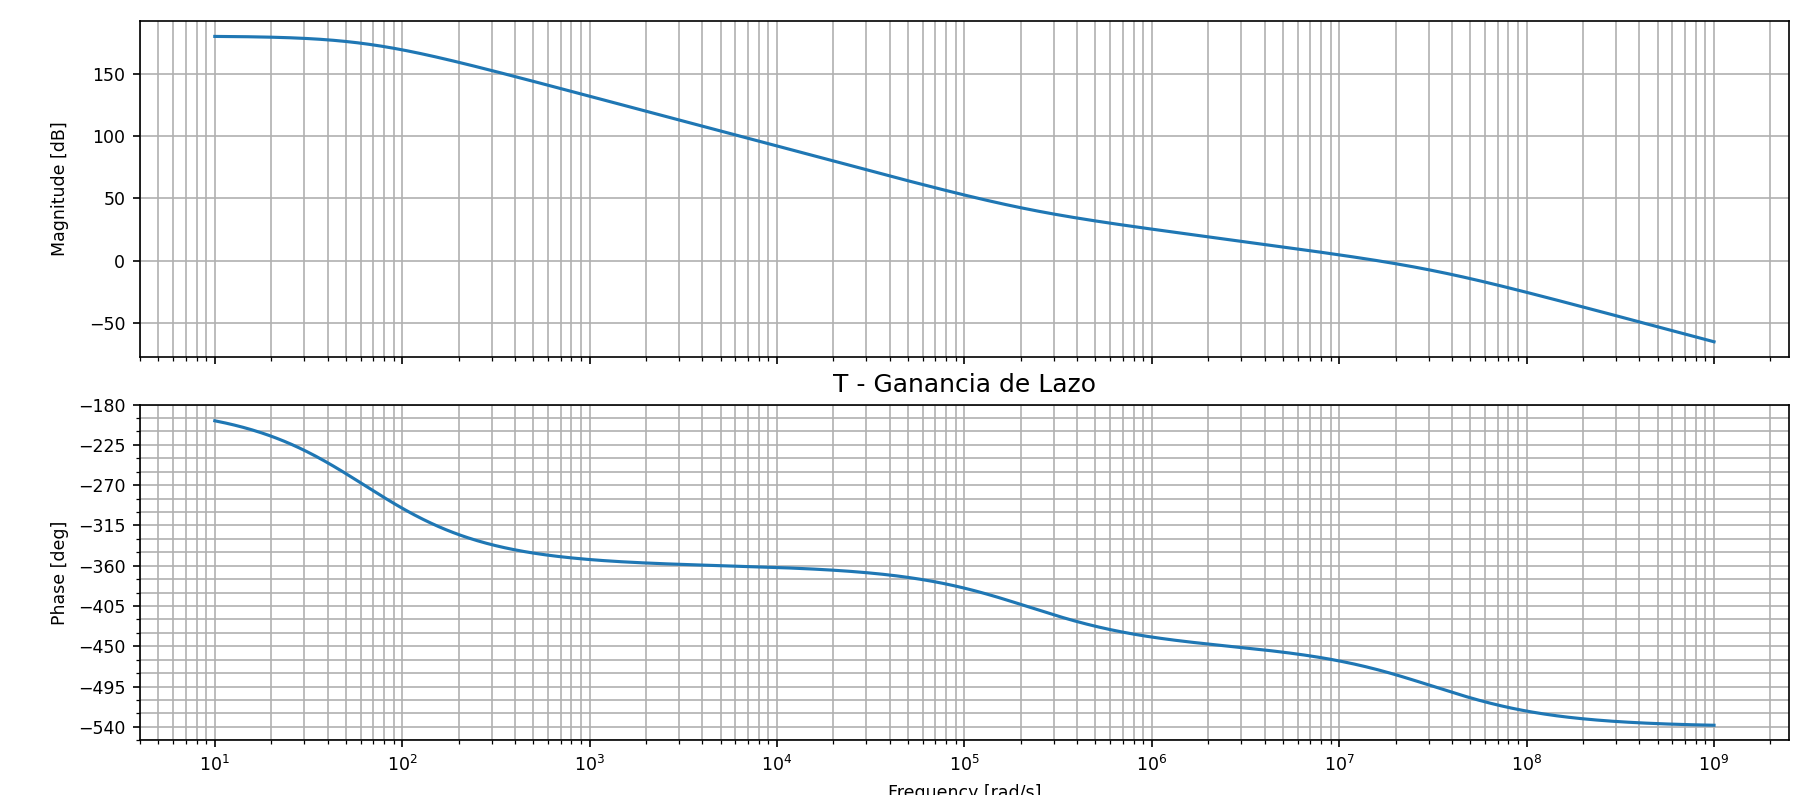
\includegraphics[width=1\linewidth]{T_py.png}
    \caption{Diagrama de Bode de $T(s)$ con $\frac{R_2}{R_1}=-1,345$}
    \label{fig:placeholder}
\end{figure}

\begin{figure}[H]
    \centering
    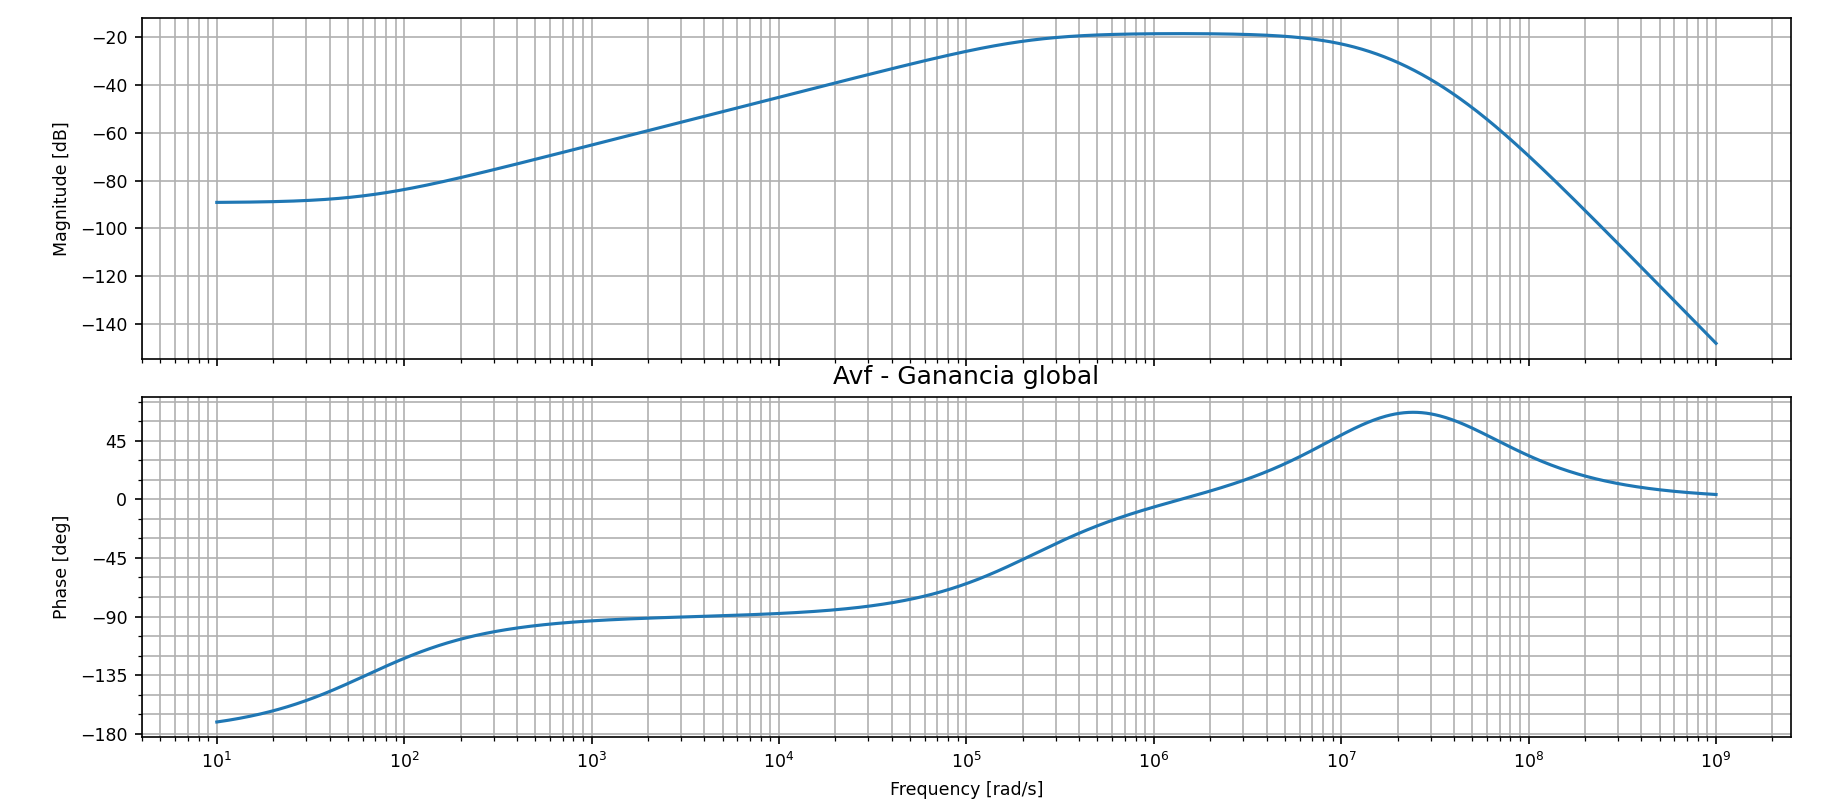
\includegraphics[width=1\linewidth]{Avf_1.png}
    \caption{Diagrama de Bode de $A{vf}(s)$ con $\frac{R_2}{R_1}=-1,345$}
    \label{fig:placeholder}
\end{figure}

El diagrama de Bode de $A_{vf}(s)$ muestra que se deja de cumplir el requerimiento de ganancia global para el valor de resistencias mencionado.

Puede notarse que la implementación de resistencias negativas en el sistema crea comportamientos indeseados en la ganancia del sistema a nivel global. Además, implementar resistencias negativas requiere de una red activa aparte y no resulta útil al contar con otras formas de compensación.

Dado que el ajuste de las resistencias $R_2$ y $R_1$ no logra que el sistema cumpla simultáneamente los requerimientos del objetivo, se puede determinar que no es una cuestión de compensación sino una limitación física de la configuración $VFA-VFA$, por lo tanto no se procedió a su simulación en LTspice ni el análisis de la respuesta al escalón, ya que éstos no aportan información adicional relevante pues el incumplimiento de los requisitos surge directamente de las limitaciones estructurales del amplificador operacional utilizado.
\\

\subsection{Conclusión parcial:}

Con el modelo adoptado para el LM324 (2 polos, $A_d(0)=100~[dB]$, $f_T=1~[MHz]$), sin realizar simplificaciones, y con la arquitectura del Circuito I, no es posible lograr simultáneamente $A_{vf}=20~[dB]$ y $M\phi \approx \ang{65,5}$ únicamente ajustando $R_1$ y $R_2$.

Si se quisiera mantener ambos amplificadores $VFA$ en el sistema y compensar el mismo de forma externa, para así obtener resultados que satisfagan los requerimientos del objetivo, se puede pensar en una red cero-polo (o múltiples de ellas) cuyas componentes cancelen el efecto de los polos y ceros creados por el segundo amplificador realimentado, de esta manera ajustar el sistema a que se comporte como fue calculado en el modelo idealizado.

\newpage
\section{Circuito II: VFA-CFA}

\subsection{Objetivo del Circuito II:}

El objetivo de este circuito es evaluar si es posible cumplir simultáneamente con una ganancia global $A_{vf}(s) = 20~[dB]$ y un Margen de Fase $M\phi = \ang{65,5}$, utilizando un amplificador $VFA$ y un amplificador $CFA$ realimentado localmente, ajustando únicamente las resistencias del lazo de realimentación local.

Se pide la misma disposición de elementos que en el circuito anterior, y llegar a una frecuencia de punto crítico $f_G=2~[MHz]$.
\\

\subsection{Modelo adoptado:}

El segundo amplificador en esta sección se cambia por un $CFA$ con las características particularmente de un LM6181:

\begin{itemize}
    \item $R_T = 2,37~[M\Omega]$
    \item $C_T = 4,8~[pF]$
    \item $f_{p1} = 14~[kHz]$        
    \item $f_{p2} = 82,3~[MHz]$
\end{itemize}
\hspace{0.5 cm}

Y como el primer amplificador sigue siendo un $VFA$, se repasan las características del LM324:

\begin{itemize}
    \item $A_d(0) = 100~[dB]$
    \item $f_T = 1~[MHz]$
    \item $f_{p3} = 10~[Hz]$        
    \item $f_{p4} = 5,06~[MHz]$
\end{itemize}
\hspace{0.5 cm}

\subsection{Análisis teórico:}

En esta arquitectura se tiene que el segundo amplificador permite ajustar el ancho de banda independientemente de la ganancia, por lo que se analiza el segundo amplificador realimentado. La función de transferencia del amplificador es la siguiente:

   \begin{equation}
        \label{eq_59}
Z_T(s) = \frac{R_T}{\left(1+\frac{s}{2\pi f_{p1}}\right)\left(1+\frac{s}{2\pi f_{p2}}\right)}
\end{equation}
    \hspace{0.5 cm}

En donde el polo $f_{p1}$ depende de los valores de $R_T$ y $C_T$ de la siguiente forma:

   \begin{equation}
        \label{eq_60}
f_{p1} = \frac{1}{2\pi C_TR_T} = 14~[kHz]
\end{equation}
    \hspace{0.5 cm}

Para llegar a la función de transferencia del $CFA$ realimentado se plantea la segunda forma de Black, junto con la ganancia de lazo cerrado ideal $A_{vfi2}(s)$ y la ganancia de lazo $T(s)$, como se muestra a continuación:

   \begin{equation}
        \label{eq_61}
A_{vf2}(s) = \frac{A_{vfi2}}{1-\frac{1}{T_2(s)}}
\end{equation}

   \begin{equation}
        \label{eq_62}
A_{vfi2} = 1+\frac{R_2}{R_1}
\end{equation}

       \begin{equation}
        \label{eq_63}
T_2(s) = -\frac{Z_T(s)}{R_2}
\end{equation}
\hspace{0.5 cm}

Se desarrolla el denominador de la ecuación (\ref{eq_61}) para simplificar la expresión de la ganancia del sistema realimentado:

       \begin{equation}
        \label{eq_64}
D(s) = 1-\frac{1}{T_2(s)} = 1+\frac{R_2}{Z_T(s)} = 1+\frac{R_2}{\frac{R_T}{\left(1+\frac{s}{2\pi f_{p1}}\right)\left(1+\frac{s}{2\pi f_{p2}}\right)}}
\end{equation}

       \begin{equation}
        \label{eq_65}
D(s) = \frac{R_2+\frac{R_T}{\left(1+\frac{s}{2\pi f_{p1}}\right)\left(1+\frac{s}{2\pi f_{p2}}\right)}}{\frac{R_T}{\left(1+\frac{s}{2\pi f_{p1}}\right)\left(1+\frac{s}{2\pi f_{p2}}\right)}}
\end{equation}

       \begin{equation}
        \label{eq_66}
D(s) = \frac{R_2\left(1+\frac{s}{2\pi f_{p1}}\right)\left(1+\frac{s}{2\pi f_{p2}}\right)+R_T}{R_T}
\end{equation}

       \begin{equation}
        \label{eq_67}
D(s) = \frac{\left(R_2+s.R_2.C_TR_T\right)\left(1+\frac{s}{2\pi f_{p2}}\right)+R_T}{R_T}
\end{equation}

       \begin{equation}
        \label{eq_68}
D(s) = \left(\frac{R_2}{R_T}+s.R_2.C_T\right)\left(1+\frac{s}{2\pi f_{p2}}\right)+1
\end{equation}
\hspace{0.5 cm}

Si se considera $R_T = 2,37~[M\Omega]~\verb|>>|~R_2$ se simplifica la misma a:

\begin{equation}
\label{eq_69}
D(s) = \left(s.R_2.C_T\right)\left(1+\frac{s}{2\pi f_{p2}}\right)+1
\end{equation}
\hspace{0.5 cm}

Y teniendo en cuenta que $f_{p2} = 82,3~[MHz]$, es posible tomar el sistema como de un solo polo en la banda de interés (cerca del punto crítico $f_G$). A continuación se muestra el denominador con esta reducción, junto con la expresión final simplificada de $A_{vf2}(s)$:

\begin{equation}
        \label{eq_70}
D(s) = 1 + sC_TR_2
\end{equation}

\begin{equation}
        \label{eq_71}
A_{vf2}(s) \approx \frac{1+\frac{R_2}{R_1}}{1 + sC_TR_2}
\end{equation}
\hspace{0.5 cm}

Tal que puede observarse que a lazo cerrado el segundo amplificador se comporta como si tuviese un solo polo móvil que depende del valor de $R_2$.

Se plantean a continuación las ganancias del sistema en conjunto necesarias para el análisis posterior, tanto la ganancia a lazo abierto $A_v(s)$ como la ganancia de lazo $T(s)$:

\begin{equation}
\label{eq_72}
A_v(s) = \frac{A_d(0)}{\left(1+\frac{s}{\omega_{p3}}\right)\left(1+\frac{s}{\omega_{p4}}\right)}\frac{A_{vfi2}}{(1 + sC_TR_2)}
\end{equation}

\begin{equation}
\label{eq_73}
T(s) = \frac{A_d(0)}{\left(1+\frac{s}{\omega_{p3}}\right)\left(1+\frac{s}{\omega_{p4}}\right)}\frac{A_{vfi2}}{(1 + sC_TR_2)}
\frac{1}{\left(1+\frac{R_f}{R_i}\right)}
\end{equation}
\hspace{0.5 cm}

\subsection{Estrategia de diseño:}

Siguiendo el proceso de la sección del circuito I, se debe encontrar una relación entre $(R_1,R_2)$ tal que se cumpla el objetivo del circuito II.

Se comienza planteando el Margen de Fase para Máxima Planicidad de Módulo a partir de la fase de $T(s)$ viendo la ecuación (\ref{eq_73}) como:

\begin{equation}
\label{eq_74}
M\phi = \ang{180} - \arctan\left(\frac{f_G}{f_{p3}}\right) - \arctan\left(\frac{f_G}{f_{p4}}\right) - \arctan\left(f_G(2\pi C_TR_2)\right) = \ang{65,5}
\end{equation}
\hspace{0.5 cm}

Tomando la frecuencia crítica del objetivo $f_G=2~[MHz]$, se despeja $R_2$:

\begin{equation}
\label{eq_75}
R_2 = \frac{\tan\left(\ang{180} - \ang{65,5}  - \arctan\left(\frac{f_G}{f_{p3}}\right) - \arctan\left(\frac{f_G}{f_{p4}}\right)\right)}{2\pi C_Tf_G} \approx 850~[\Omega]
\end{equation}
\hspace{0.5 cm}

A partir de este resultado, con la ayuda de un código de Python que se encuentra en el Anexo (\ref{codigo5}), se realizó un barrido de valores de $R_1$ que permitan encontrar el valor exacto tal que $f_G = 2~[MHz]$. Se muestra a continuación la gráfica que genera el código:

\begin{figure}[H]
    \centering
    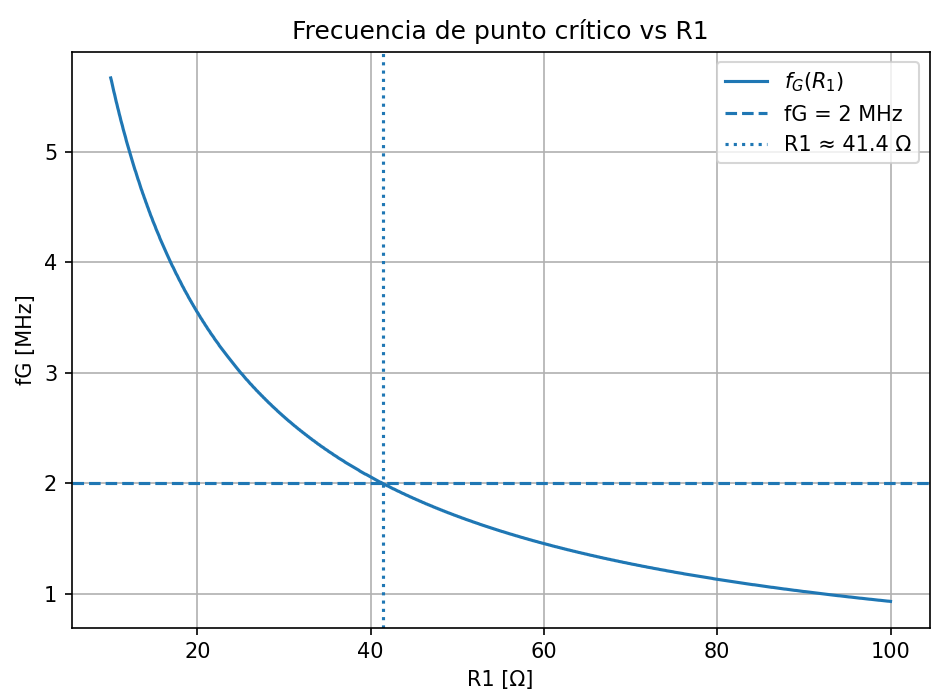
\includegraphics[width=0.7\linewidth]{fG_vs_R1_C2.png}
    \caption{$f_G$ respecto al barrido de $R_1$}
    \label{fig:placeholder}
\end{figure}

Por lo tanto el valor de $R_1$ que verifica $f_G = 2~[MHz]$ es:

\begin{equation}
\label{eq_76}
R_1 = 41,4~[\Omega]
\end{equation}
\hspace{0.5 cm}

Con la ayuda de un código de Python que se encuentra en el Anexo (\ref{codigo6}) se hizo posible verificar los requerimientos del sistema, los cuales se recuerdan a continuación:

\begin{itemize}
    \item $A_{vf} = 20~[dB]$
    \item $M{\phi} =$ \ang{65,5}        
    \item $f_G = 2~[MHz]$
\end{itemize}

El código mencionado calcula y grafica los diagramas de Bode de $T(s)$ y $A_{vf}(s)$, esta vez sin simplificaciones y con los valores de $R_1$ y $R_2$ establecidos. Se presenta a continuación la información:

\begin{figure}[H]
    \centering
    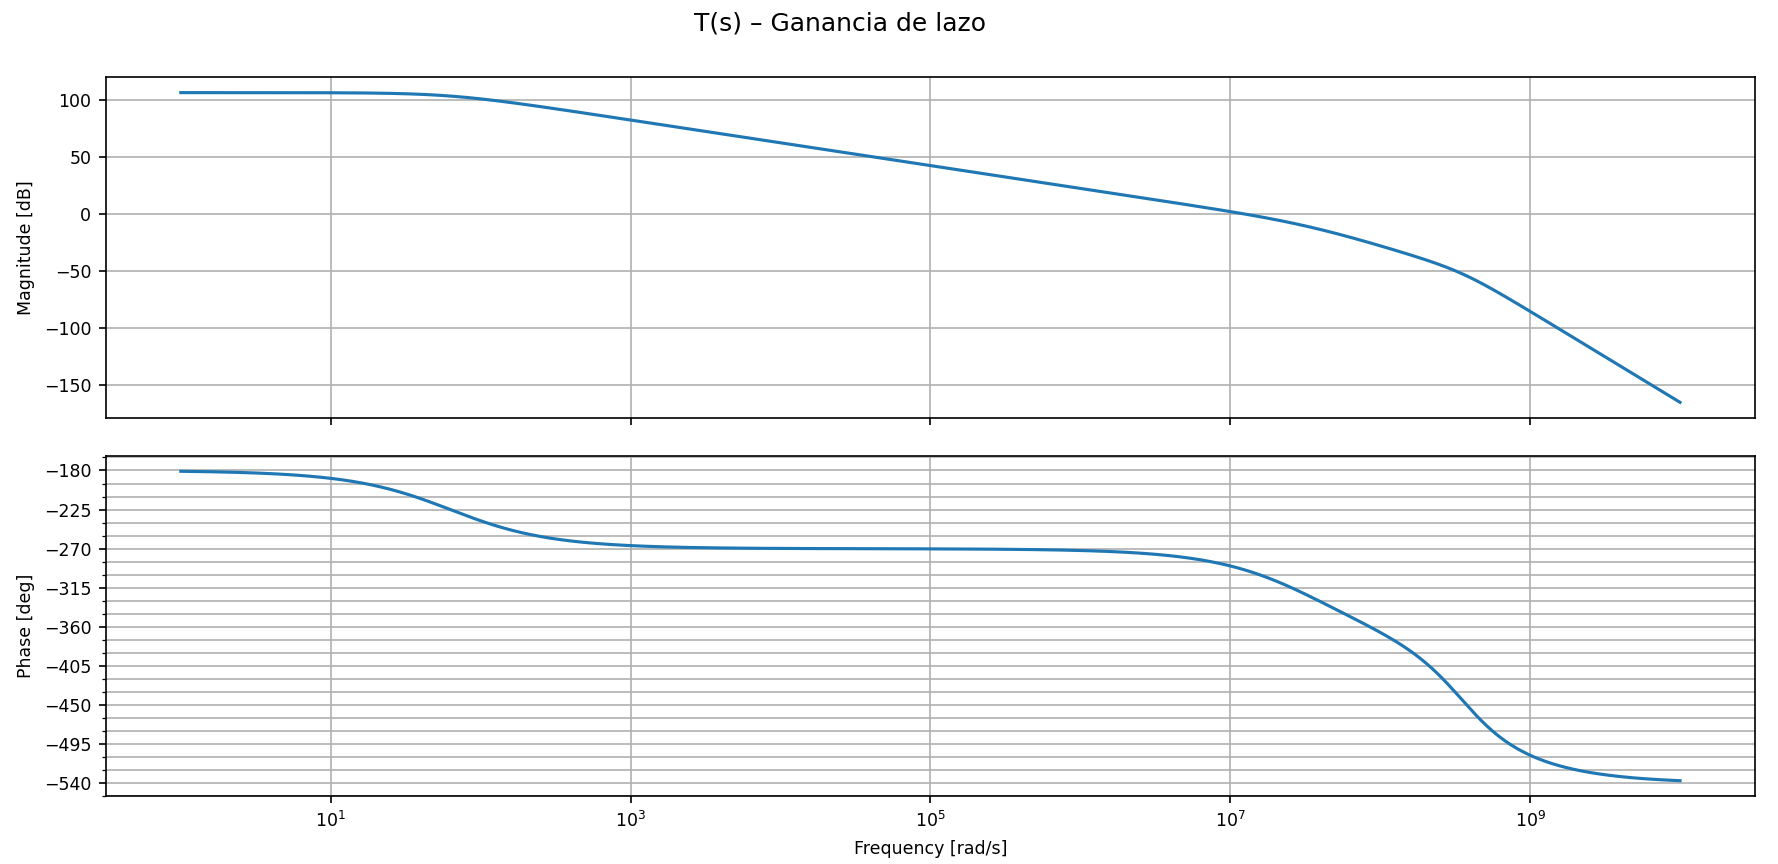
\includegraphics[width=1\linewidth]{Bode_T_C2.png}
    \caption{$T(s)$ con $R_1 = 41,4~[\Omega]$}
    \label{fig:placeholder}
\end{figure}

\begin{figure}[H]
    \centering
    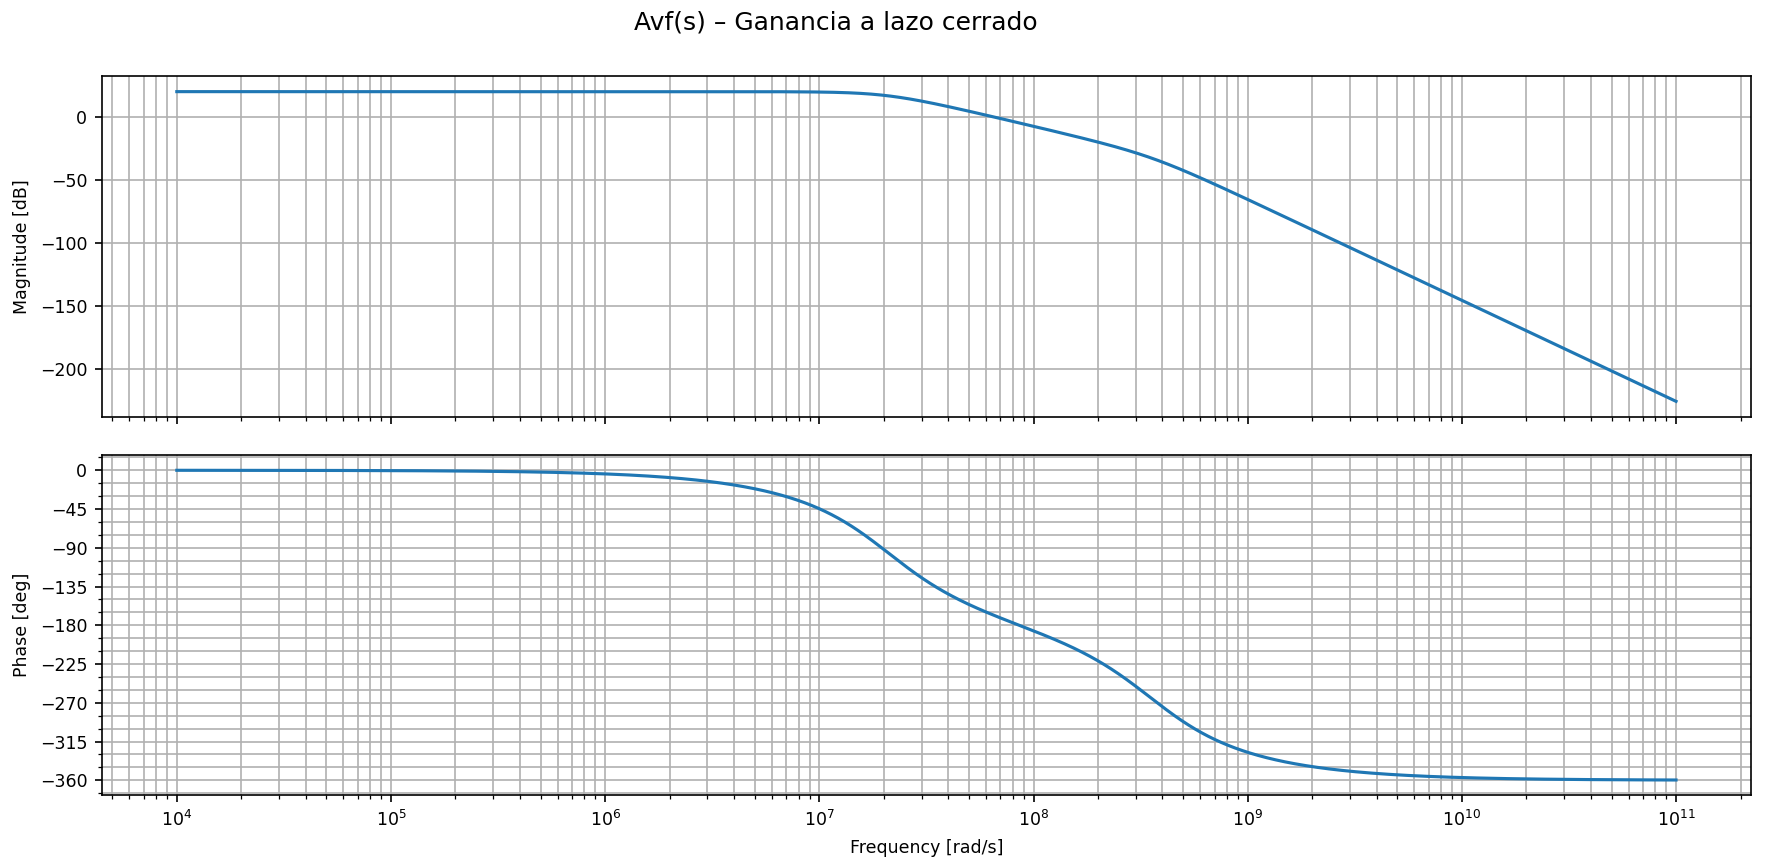
\includegraphics[width=1\linewidth]{Bode_Avf_C2.png}
    \caption{$A_{vf}(s)$ con $R_1 = 41,4~[\Omega]$}
    \label{fig:placeholder}
\end{figure}

Se ve en el Bode de $T(s)$ el cruce por $0[dB]$ en $\omega_G = 1,25\,.\,10^7[\frac{rad}{s}]$, por lo que:

\begin{equation}
\label{eq_77}
f_G = \frac{\omega_G}{2\pi} = 1,989~[MHz] \approx 2~[MHz]
\end{equation}
\hspace{0.5 cm}

En el gráfico de Bode de $A_{vf}(s)$ se observan los $20~[dB]$ requeridos, con una caída de $3~[dB]$ en $\omega_p = 2,02\,.\,10^7~[\frac{rad}{s}]$, por lo tanto puede escribirse:

\begin{equation}
\label{eq_78}
f_p = \frac{\omega_p}{2\pi} = 3,2~[MHz]
\end{equation}
\hspace{0.5 cm}

Además el código devuelve el Margen de Fase utilizando la función \texttt{margin} del paquete de \texttt{control} de Python. Al utilizarlo en la expresión de $T(s)$ y resulta:

\begin{equation}
\label{eq_79}
M\phi = \ang{65,48}
\end{equation}
\hspace{0.5 cm}

Lo cual es coherente con el diagrama de Bode de $T(s)$ ya que se observa una fase de $\phi \approx \ang{-295}$, lo cual está a $\ang{65}$ de los $\ang{360}$ que son condición para la inestabilidad del sistema.

Se implementó un código de Python que se encuentra en el Anexo (\ref{codigo7}), que grafica la respuesta al escalón de $A_{vf}(s)$, para estimar el Margen de Fase del sistema utilizando:

\begin{itemize}
    \item El Valor Máximo de la respuesta $y_{max}$
    \item El Sobrepasamiento $M_p$        
    \item El Factor de Amortiguamiento $\zeta$
\end{itemize}

Para hacerlo utiliza las siguientes relaciones entre parámetros:


\begin{equation}
\label{eq_80}
M_p = \frac{y_{max} - y_{\infty}}{y_{\infty}}
\end{equation}

\begin{equation}
\label{eq_81}
M_p = e^{-\frac{\pi~\zeta}{\sqrt{1-\zeta^2}}}
\end{equation}

\begin{equation}
\label{eq_82}
M\phi = \arctan{\frac{2\zeta}{\sqrt{1 + 4\zeta^4}-2\zeta^2}}
\end{equation}
\hspace{0.5 cm}

A continuación se muestra el gráfico de la respuesta al escalón:

\begin{figure}[H]
    \centering
    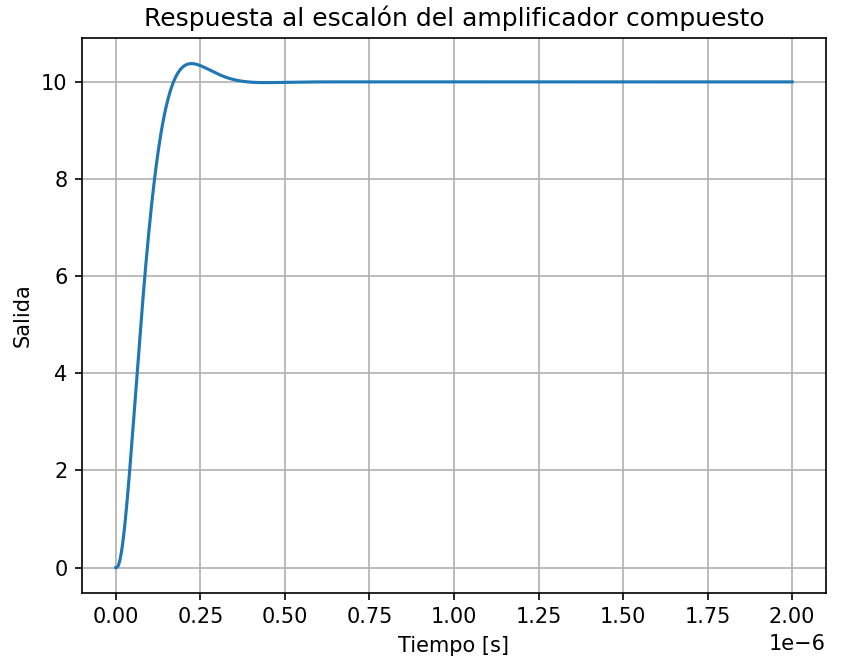
\includegraphics[width=0.8\linewidth]{Step_C2.png}
    \caption{Respuesta al escalón del circuito II}
    \label{fig:placeholder}
\end{figure}

Mientras que el código devuelve los siguientes valores:

\begin{equation}
\label{eq_83}
y_{max} =  10,373
\end{equation}

\begin{equation}
\label{eq_84}
M_p =  3,73~\%
\end{equation}

\begin{equation}
\label{eq_85}
\zeta =  0,723
\end{equation}

\begin{equation}
\label{eq_86}
M\phi =  \ang{66,34}
\end{equation}
\hspace{0.5 cm}

Se hizo uso de un código de Python que se encuentra en el Anexo (\ref{codigo8}), para calcular los polos y la ganancia estática de $A_{vf}(s)$ sin la simplificación hecha en su denominador, los cuales resultaron:

\begin{equation}
\label{eq_87}
f_{p5} = 56,797~[MHz]
\end{equation}

\begin{equation}
\label{eq_88}
f_{p6} = 56,797~[MHz]
\end{equation}

\begin{equation}
\label{eq_89}
f_{p7} = 3,2939~[MHz]
\end{equation}

\begin{equation}
\label{eq_90}
f_{p8} = 3,2939~[MHz]
\end{equation}

\begin{equation}
\label{eq_91}
K = 9,9999~[veces]
\end{equation}
\hspace{0.5 cm}

Se tienen dos polos dobles, en $3,3~[MHz]$ y $56,8~[MHz]$, y el valor de $K$ vuelve a verificar el requerimiento cumplido. También es posible verificar el valor de frecuencia de la caída de $-3~[dB]$ que anteriormente se logró ver en el diagrama de Bode y se determinó que eran $3,2~[MHz]$.
\\

\subsection{Conclusión parcial:}
Se lograron determinar los valores de los componentes del lazo del $CFA$ para cumplir correctamente con los requerimientos de ganancia global, Margen de Fase y frecuencia de punto crítico.

La verificación tanto mediante simulaciones en dominio de la frecuencia como la estimación a partir de la respuesta al escalón mostraron que el sistema presenta una ganancia a lazo cerrado de 10 veces, una frecuencia de cruce coherente con la especificación y un margen de fase cercano a 65,5°, en concordancia con el criterio de Máxima Planicidad de Módulo.
\\

\subsection{Simulación:}

Se dispuso el siguiente circuito en el programa LTspice para analizar su comportamiento. Los modelos de los amplificadores se encuentran en el Anexo (\ref{modelo_VFA}) y (\ref{modelo_CFA}):

\begin{figure}[H]
    \centering
    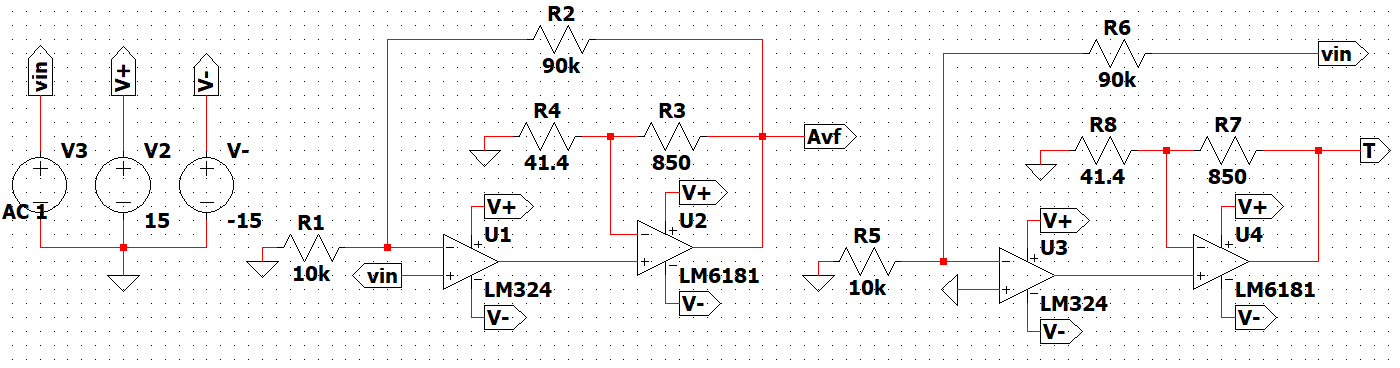
\includegraphics[width=1\linewidth]{Spice_C2.png}
    \caption{Diagrama circuital en LTspice}
    \label{fig:placeholder}
\end{figure}

A partir del mismo se graficaron los diagramas de Bode de $A_{vf}(s)$ y $T(s)$ tal que sea posible evaluar los valores de interés. A continuación se muestran ambos, seguidos de los datos:

\begin{figure}[H]
    \centering
    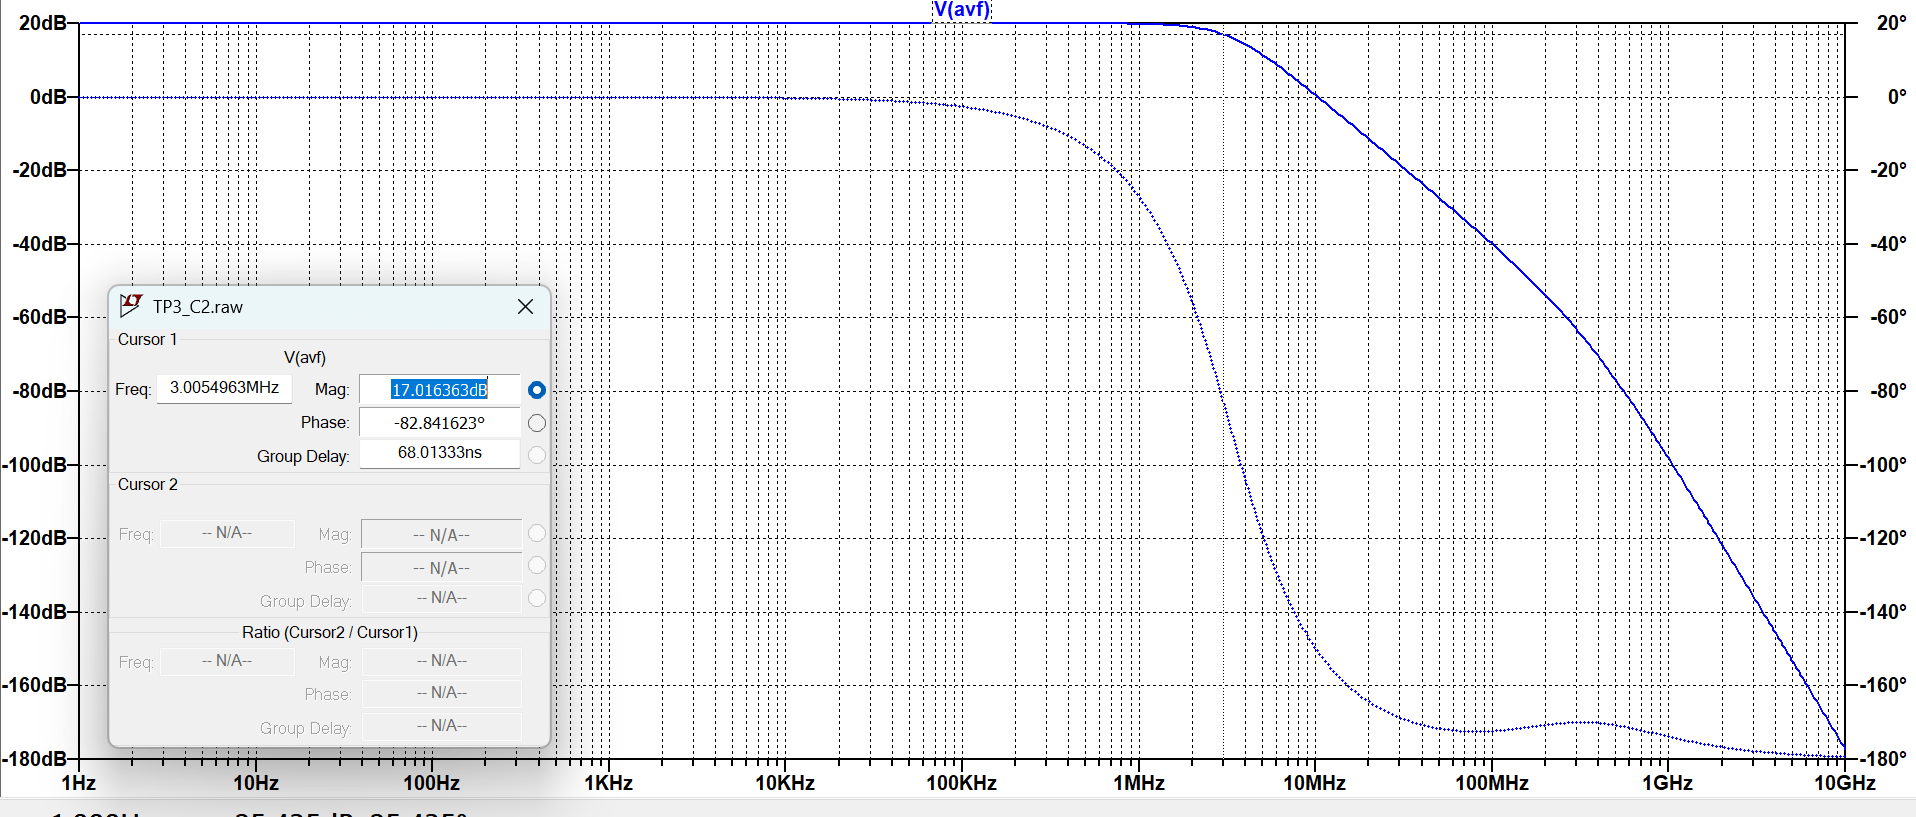
\includegraphics[width=1\linewidth]{Bode_Spice_Avf_C2.png}
    \caption{Diagrama de Bode de $A_{vf}(s)$}
    \label{fig:placeholder}
\end{figure}

En el cual puede verse correctamente que se logra el valor de ganancia global requerido, además de la frecuencia de la caída de $-3~[dB]$ del sistema en $f_p = 3~[MHz]$. También puede medirse la frecuencia a la que el sistema está en $\ang{-90}$, en la cual está el polo doble $f_{p7}=f_{p8}=3,3~[MHz]$. Sin embargo el otro polo doble que calculó el código de Python del Anexo (\ref{codigo8}) no logra verse en el diagrama (el que se muestra en las ecuaciones (\ref{eq_87}) y (\ref{eq_88})).
\\

\begin{figure}[H]
    \centering
    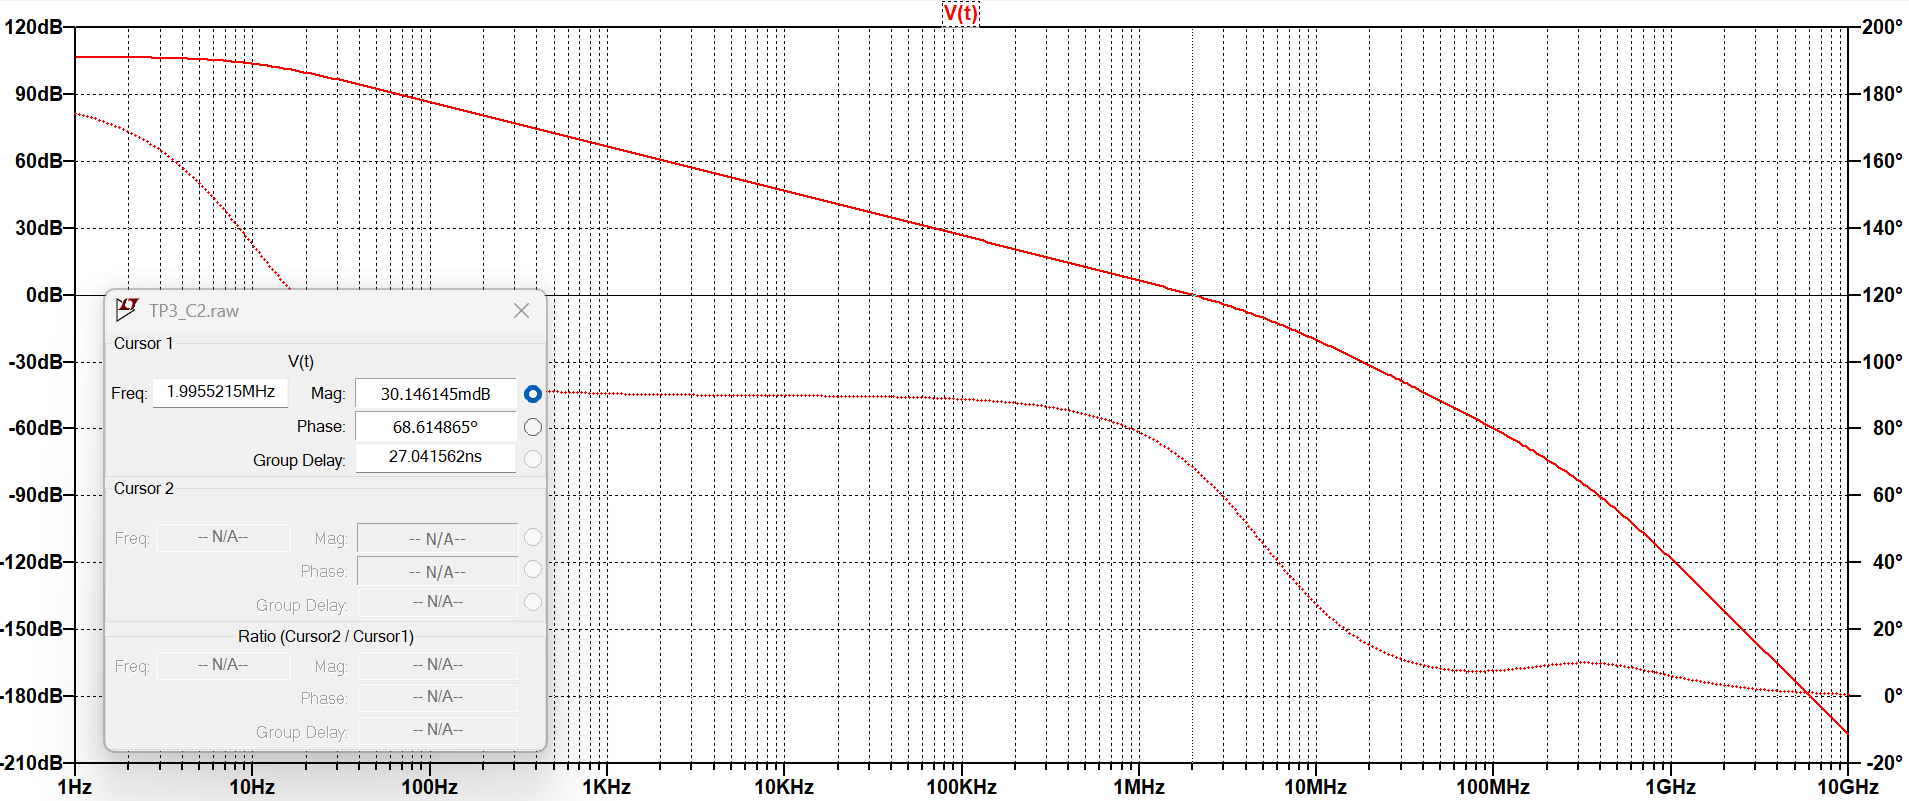
\includegraphics[width=1\linewidth]{Bode_Spice_T_C2.png}
    \caption{Diagrama de Bode de $T(s)$}
    \label{fig:placeholder}
\end{figure}

En donde el cursor marca el valor de $\left|T(s)\right|=0~[dB]$ en la frecuencia que corresponde al punto crítico y logra verse $f_G=2~[MHz]$. También se aprecia en ese punto una fase de $\phi=\ang{68,61}$.

Para este apartado, es posible concluir que el circuito se comporta tal y como fue diseñado, calculado y analizado teóricamente, logrando alcanzar los objetivos propuestos para el mismo y siendo coherente con los resultados obtenidos anteriormente por medio de distintos caminos.

\newpage
\section{Circuito III: VFA - Red Cero-Polo - CFA}

\subsection{Objetivo del Circuito III:}

Se requiere implementar el circuito II, agregando una red cero-polo a la salida del $VFA$ para cancelar su polo más lejano y presenciar una mejora en el Margen de Fase respecto del caso anterior.

El polo que genera la red deberá ser colocado una octava por encima de su cero, y también debe retocarse la ganancia del $CFA$ para compensar la atenuación que introduce la red pasiva.
\\

\subsection{Modelo adoptado:}

Siendo que el circuito III se basa en el circuito anterior, los modelos adoptados para éste se repiten. Véase el apartado $(4\,.\,2)$.
\\

\subsection{Estrategia de diseño:}

La función de transferencia de la red, que puede verse en las ecuaciones (\ref{eq_22}) y (\ref{eq_26}), son tal que para cancelar el segundo polo del $VFA$ debe cumplirse:

\begin{equation}
\label{eq_92}
f_{zc} = 5,06~[MHz]
\end{equation}

\begin{equation}
\label{eq_93}
f_{pc} = 10,12~[MHz]
\end{equation}
\hspace{0.5 cm}

Recordando las ecuaciones (\ref{eq_23}), (\ref{eq_24}) y (\ref{eq_25}), se elige arbitrariamente el valor del capacitor $C_x$ tal que se puedan despejar los valores de resistencias de las ecuaciones anteriores. Por lo tanto, se establece:

\begin{equation}
\label{eq_94}
C_x = 10~[pF]
\end{equation}
\hspace{0.5 cm}

Entonces despejando $R_x$ de la ecuación (\ref{eq_24}) se obtiene:

\begin{equation}
\label{eq_95}
R_x = \frac{1}{\omega_{zc}\,C_x} = \frac{1}{2 \pi \, 5,06~.~10^6~[Hz]~.\,10^{-11}~[F]} = 3145,355 ~[\Omega]
\end{equation}
\hspace{0.5 cm}

Luego, para despejar $R_y$ hizo la relación entre las expresiones de $\omega_{pc}$ y $\omega_{zc}$, como se muestra a continuación:

\begin{equation}
\label{eq_96}
\frac{\omega_{pc}}{\omega_{zc}} = \frac{\frac{1}{C_x(R_x//R_y)}}{\frac{1}{C_xR_x}} = \frac{C_xR_x}{C_x(R_x//R_y)}= \frac{C_xR_x}{C_x\frac{R_xR_y}{R_x + R_y}} = \frac{R_x + R_y}{R_y}
\end{equation}
\hspace{0.5 cm}

Y conociendo que $\omega_{pc}$ está una octava más arriba que $\omega_{zc}$, puede determinarse:

\begin{equation}
\label{eq_97}
\frac{\omega_{pc}}{\omega_{zc}} = 2 = 1+\frac{R_x}{R_y}
\end{equation}

\begin{equation}
\label{eq_98}
R_y =R_x = 3145,355~[\Omega]
\end{equation}
\hspace{0.5 cm}

A partir de la obtención de los valores de cada componente se puede calcular además la atenuación que genera la red como se ve en la ecuación (\ref{eq_23}):

\begin{equation}
   \label{eq_99}
   A_C(0) = \frac{R_y}{R_y+R_x} = 0,5~[veces] = -6~[dB]
\end{equation}
\hspace{0.5 cm}

Como la red pasiva hace caer el nivel de la señal a la mitad, se debe duplicar la ganancia en la siguiente etapa tal que se compense esta caída. En la sección anterior se definió $A_{vfi2} = 1+\frac{R_2}{R_1} = 21,5~[veces]$, por lo que para este circuito se debe lograr:

\begin{equation}
   \label{eq_100}
   A_{vfi2} = 1+\frac{R_2}{R_1} = 2\,.\,(21,5)=43~[veces]
\end{equation}
\hspace{0.5 cm}

Para que no varíe el polo móvil del $CFA$ se ajusta $R_1$ de la siguiente manera:

\begin{equation}
   \label{eq_101}
   R_1 = \frac{850~[\Omega]}{43-1} = 20,238~[\Omega]
\end{equation}
\hspace{0.5 cm}

Se hizo uso de un código de Python que se encuentra en el Anexo (\ref{codigo9}), el cual toma el polo, el cero y la ganancia estática de una función de transferencia valuada con los componentes calculados ($C_x$, $R_x$ y $R_y$). Ésta devuelve los siguientes valores:

\begin{equation}
\label{eq_102}
f_{zc} = 5,06~[MHz]
\end{equation}

\begin{equation}
\label{eq_103}
f_{pc} = 10,12~[MHz]
\end{equation}

\begin{equation}
\label{eq_104}
K_{A_c} = 0,5~[veces]
\end{equation}
\hspace{0.5 cm}

El código (\ref{codigo9}) también grafica un diagrama de Bode de la red pasiva, se muestra a continuación:

\begin{figure}[H]
    \centering
    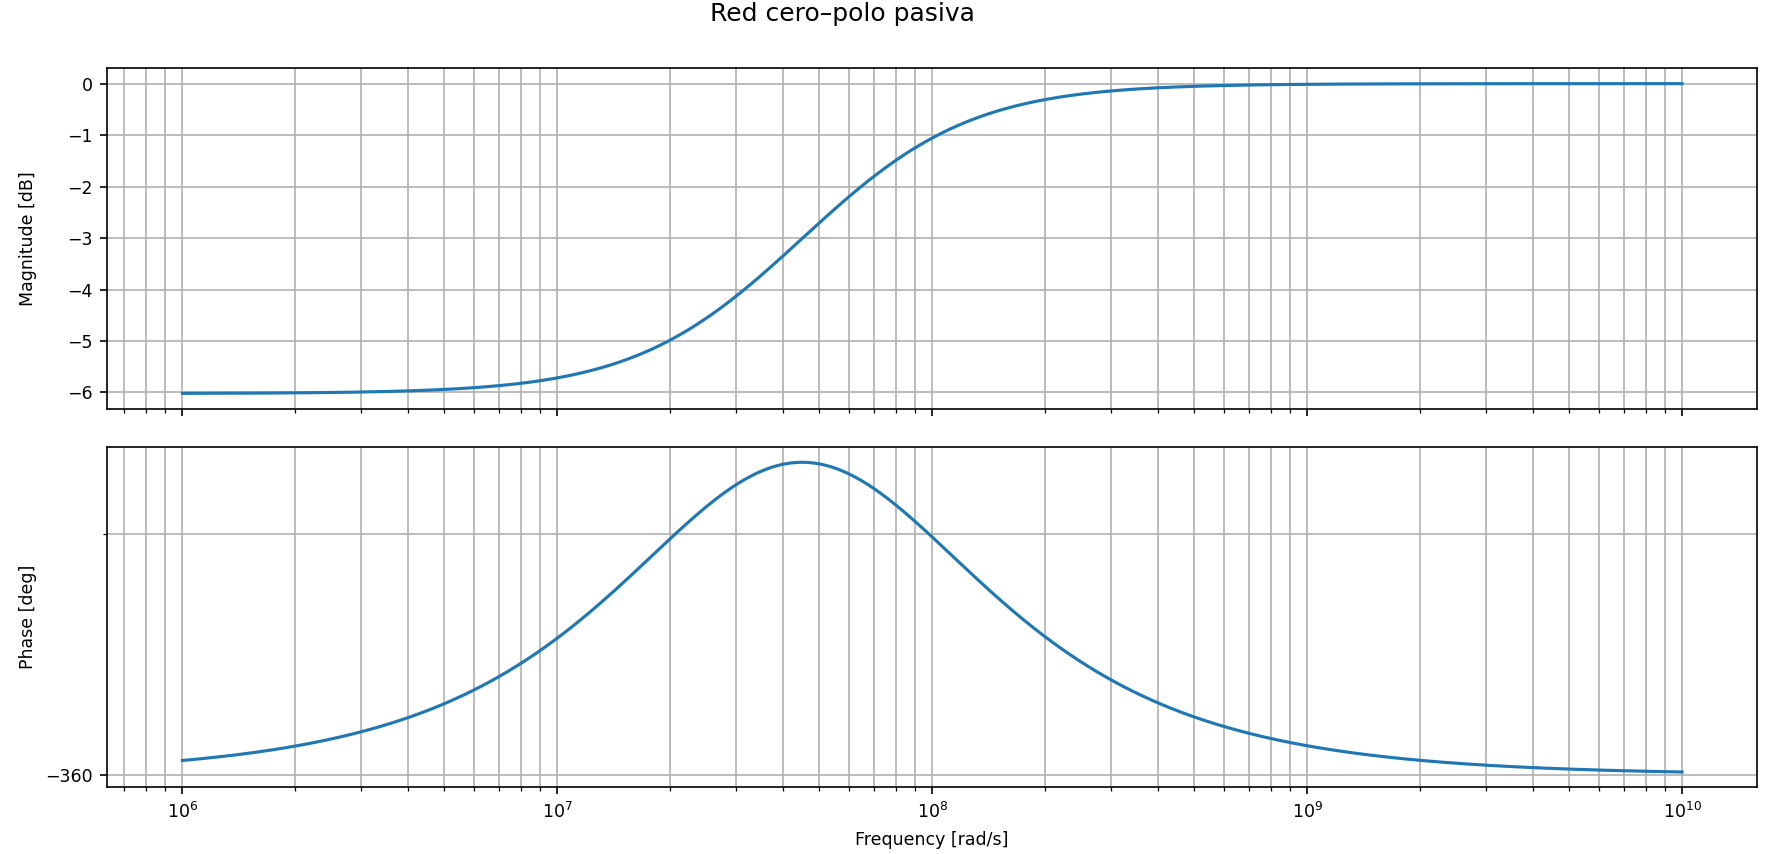
\includegraphics[width=1\linewidth]{Bode_RC.png}
    \caption{Diagrama de Bode de la red cero-polo}
    \label{fig:placeholder}
\end{figure}

En el mismo es posible ver la atenuación a frecuencias menores, y la dinámica de la existencia de un cero seguido de un polo en módulo y fase.

Posteriormente, se hizo uso de un código de Python que se encuentra en el Anexo (\ref{codigo10}) que agrega la dinámica de comportamiento del $VFA$ y del $CFA$ junto a la red cero-polo. Esto para revisar los polos que restan luego del ajuste de componentes realizado. 

El código devuelve los polos y ceros existentes en el sistema total a lazo cerrado, además de la ganancia estática, y grafica el diagrama de Bode del mismo y de la ganancia de lazo $T(s)$. 

A continuación se muestran los 
diagramas y posteriormente los resultados que arroja el programa:

\begin{figure}[H]
    \centering
    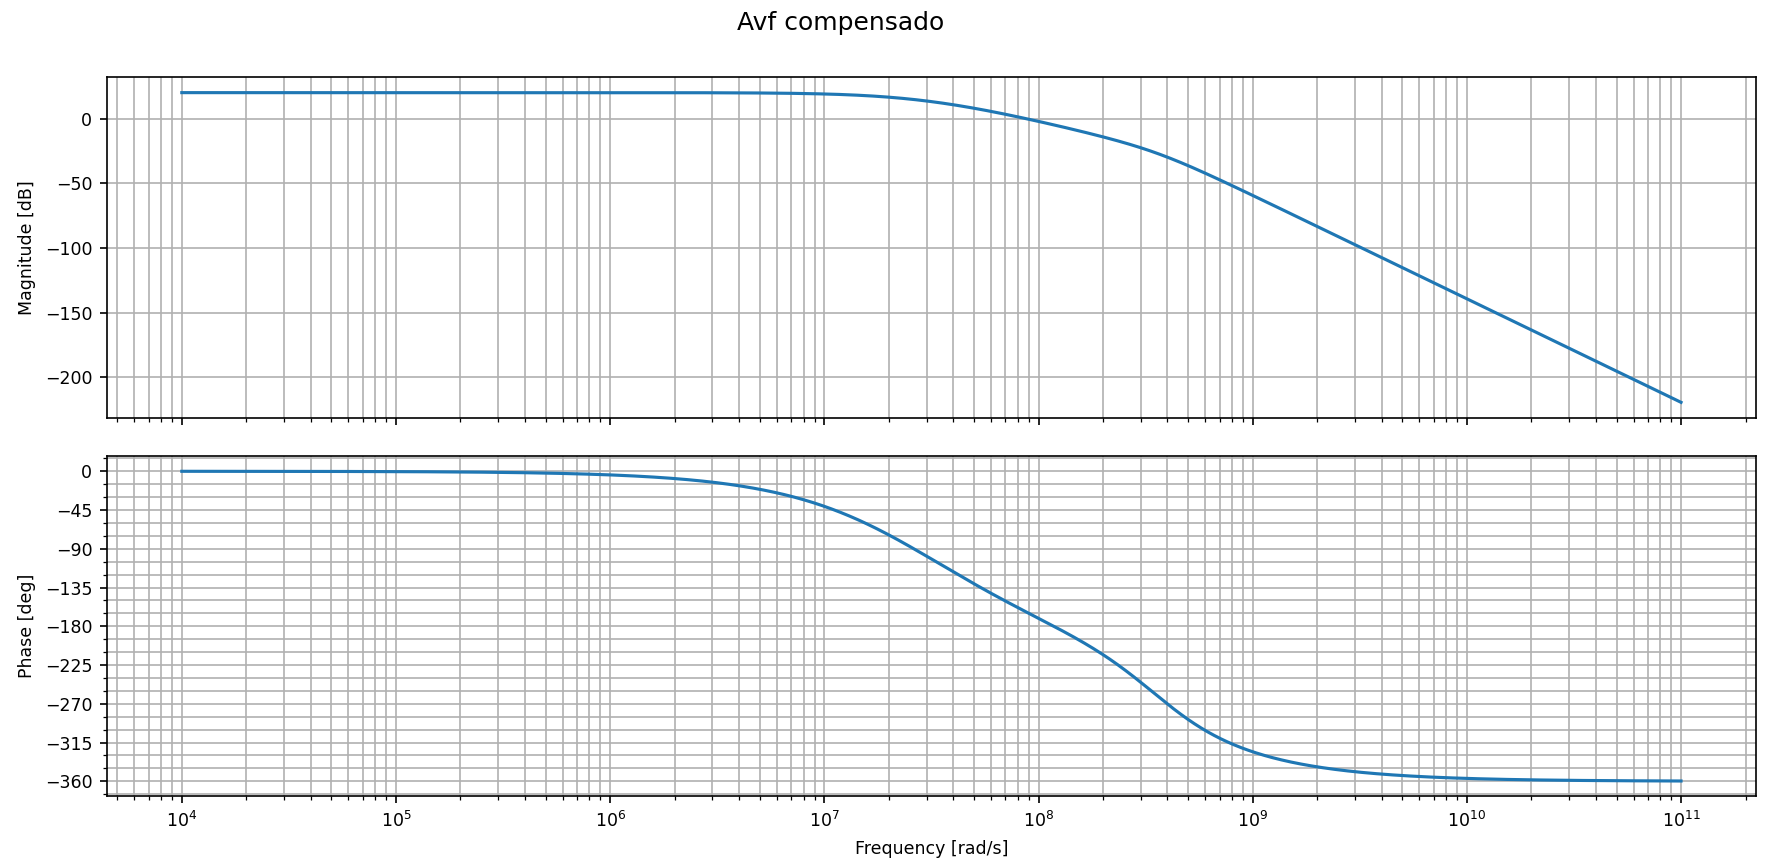
\includegraphics[width=1\linewidth]{Bode_Avf_C3.png}
    \caption{Diagrama de Bode del sistema $A_{vf}(s)$}
    \label{fig:placeholder}
\end{figure}

\begin{figure}[H]
    \centering
    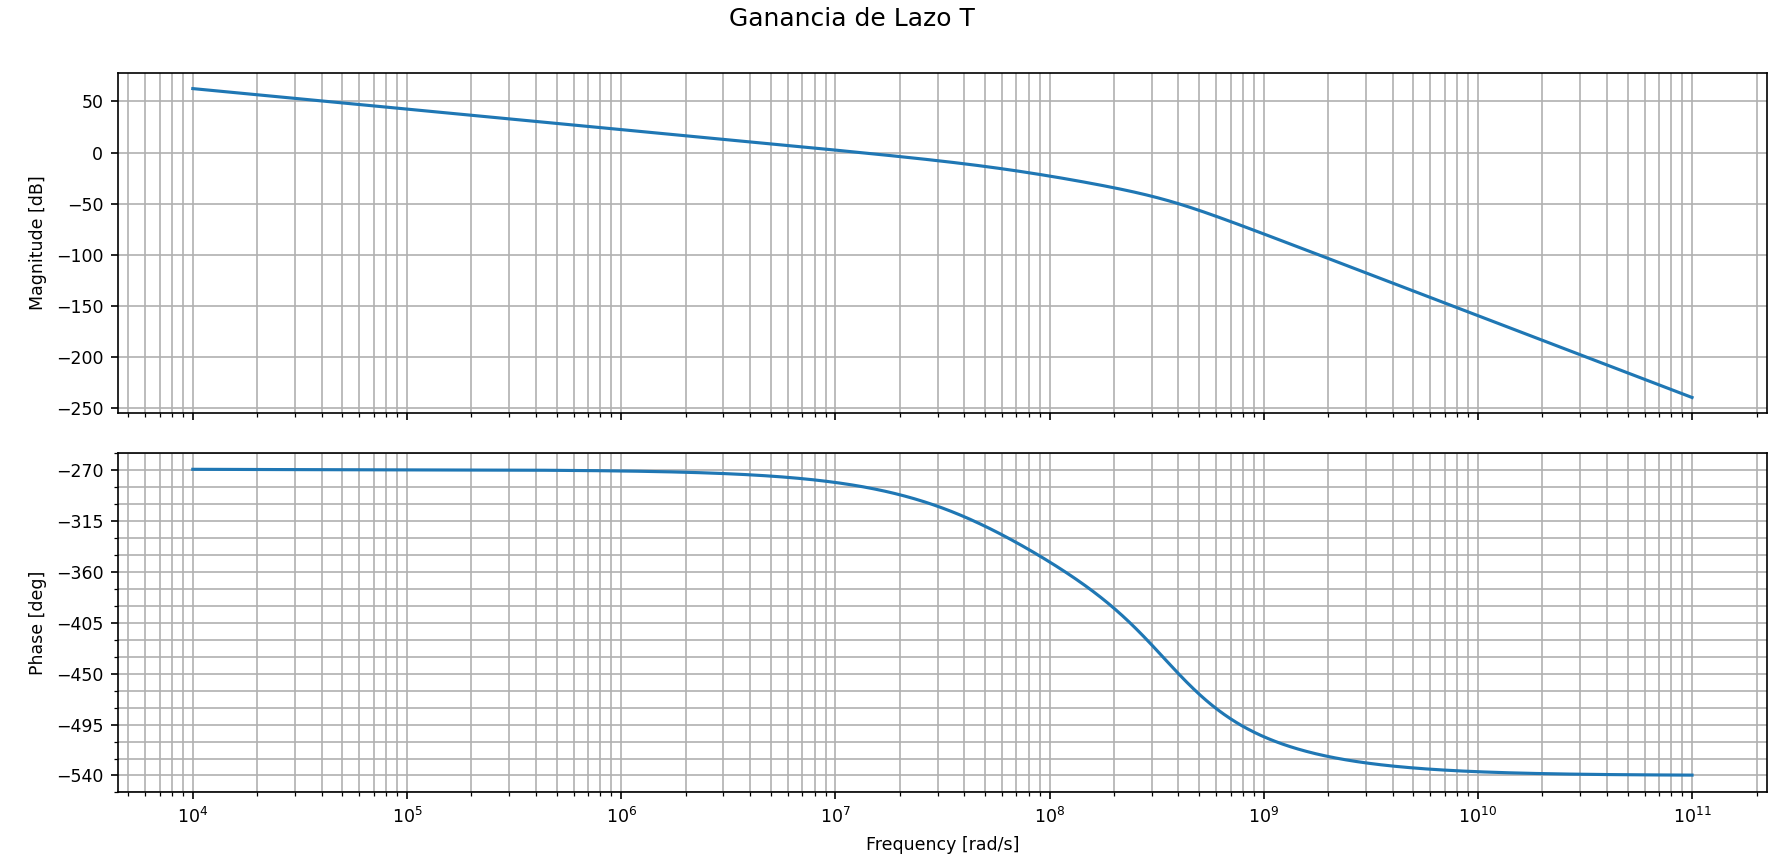
\includegraphics[width=1\linewidth]{Bode_T_C3_1.png}
    \caption{Diagrama de Bode del sistema $T(s)$}
    \label{fig:placeholder}
\end{figure}

\begin{equation}
\label{eq_105}
f_{p1} = 56,9~[MHz]
\end{equation}

\begin{equation}
\label{eq_106}
f_{p2} = 56,9~[MHz]
\end{equation}

\begin{equation}
\label{eq_107}
f_{p3} = 5,712~[MHz]
\end{equation}

\begin{equation}
\label{eq_108}
f_{p4} = 3,78~[MHz]
\end{equation}

\begin{equation}
\label{eq_109}
K_{A_{vf}} = 9,9999~[veces]
\end{equation}
\hspace{0.5 cm}

Puede determinarse con el cursor sobre el diagrama de Bode de $A_{vf}(s)$ que la caída de $-3~[dB]$ se encuentra en $f_p = 2,9~[MHz]$. Y de la misma forma en el diagrama de Bode de $T(s)$ se determina que el punto crítico se encuentra en $f_G = 2,1~[MHz]$

El código del Anexo (\ref{codigo10}) también calcula el Margen de Fase de la misma forma que el código del Anexo (\ref{codigo6}). Con el sistema actual éste devuelve un Margen de fase de:

\begin{equation}
\label{eq_110}
M\phi = \ang{75,17}
\end{equation}
\hspace{0.5 cm}

Al cancelar el polo del $VFA$ en $5,06~[MHz]$ y agregar uno una octava más arriba, se agrega fase positiva alrededor del punto crítico $f_G = 2,1~[MHz]$, lo cual inevitablemente aumenta el Margen de Fase $M\phi$ respecto del circuito anterior. Si bien se excede el Margen de Fase requerido, representa una mejora en términos de estabilidad del sistema y una mayor amortiguación de la respuesta como se logra ver en la respuesta al escalón que grafica el código de Python que se encuentra en el Anexo (\ref{codigo11}) y se muestra a continuación:

\begin{figure}[H]
    \centering
    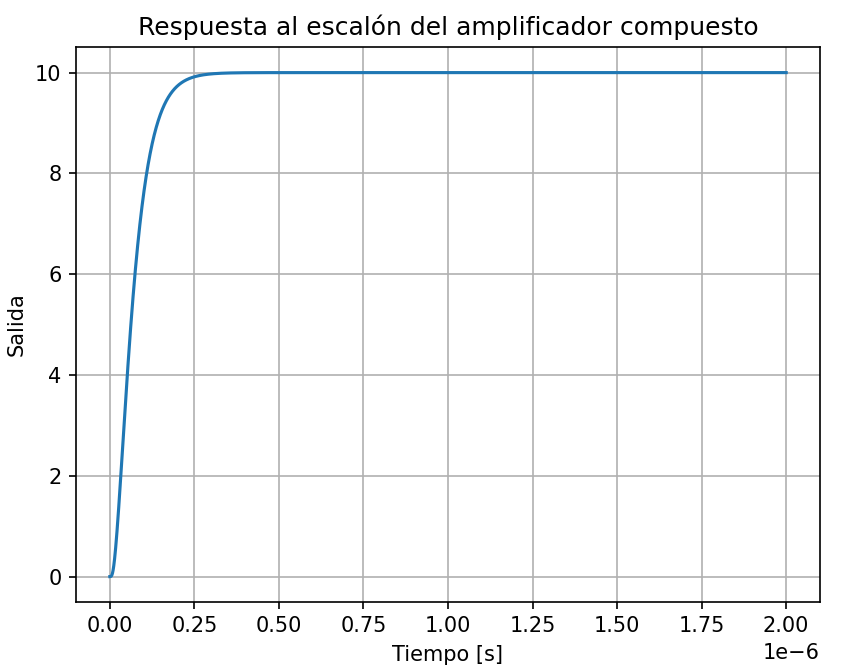
\includegraphics[width=0.7\linewidth]{Step_C3_1.png}
    \caption{Respuesta al escalón del circuito III amortiguado}
    \label{fig:placeholder}
\end{figure}

\subsubsection{Ajuste de $R_2$ y $R_1$:}

Si se quiere retocar el Margen de Fase, se debe acercar $f_G$ a un punto en frecuencia donde la fase de $T(s)$ se acerce a $\ang{180}$. En este caso, para lograrlo se debe aumentar el valor de $f_G$, modificando el valor de $R_2$ para ajustar el polo y la ganancia del $CFA$. Se utilizó la misma expresión que la ecuación (\ref{eq_73}), (\ref{eq_74}) y (\ref{eq_75}) para despejar $R_2$ fijando nuevamente un valor de $f_G = 2~[MHz]$.

\begin{equation}
\label{eq_111}
T(s) = \frac{A_d(0)}{\left(1+\frac{s}{\omega_{p3}}\right)\left(1+\frac{s}{\omega_{p4}}\right)}\frac{A_c(0)\left(1+\frac{s}{\omega_{zc}}\right)}{\left(1+\frac{s}{\omega_{pc}}\right)}\frac{A_{vfi2}}{(1 + sC_TR_2)}
\frac{1}{\left(1+\frac{R_f}{R_i}\right)}
\end{equation}

\begin{equation}
\label{eq_112}
T(s) = \frac{A_d(0)}{\left(1+\frac{s}{\omega_{p3}}\right)}\frac{A_c(0)}{\left(1+\frac{s}{\omega_{pc}}\right)}\frac{A_{vfi2}}{(1 + sC_TR_2)}
\frac{1}{\left(1+\frac{R_f}{R_i}\right)}
\end{equation}

\begin{equation}
\label{eq_113}
M\phi = \ang{180} - \arctan\left(\frac{f_G}{f_{p3}}\right) - \arctan\left(\frac{f_G}{f_{pc}}\right) - \arctan\left(f_G(2\pi C_TR_2)\right) = \ang{65,5}
\end{equation}

\begin{equation}
\label{eq_114}
R_2 = \frac{\tan\left(\ang{180} - \ang{65,5}  - \arctan\left(\frac{f_G}{f_{p3}}\right) - \arctan\left(\frac{f_G}{f_{pc}}\right)\right)}{2\pi C_Tf_G} \approx 3925,46~[\Omega]
\end{equation}
\hspace{0.5 cm}

Y posteriormente se realizó un barrido del valor de $R_1$ para posicionar correctamente el punto crítico en $f_G = 2~[MHz]$, para esto se hizo uso de un código de Python que se encuentra en el Anexo (\ref{codigo12}) que aplica las mismas funciones que el código del Anexo (\ref{codigo5}) utilizado anteriormente, pero con el sistema actual. A continuación se muestra el gráfico del barrido:

\begin{figure}[H]
        \centering
    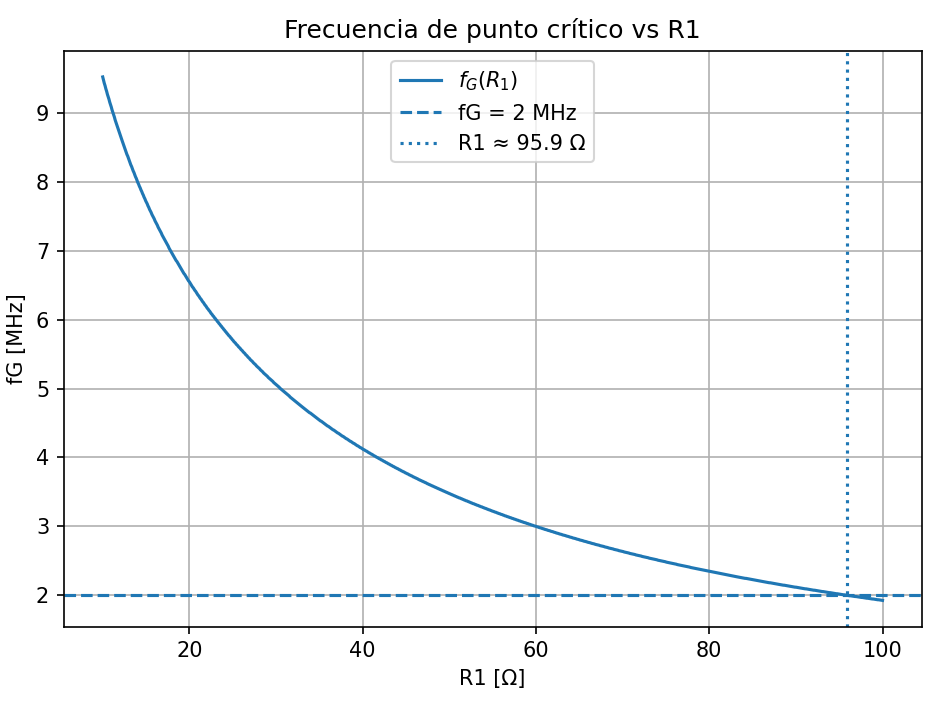
\includegraphics[width=0.7\linewidth]{Barrido_R1_C3.png}
    \caption{$f_G$ respecto al barrido de $R_1$n}
    \label{fig:placeholder}
\end{figure}

Por lo tanto el valor de $R_1$ que verifica $f_G = 2~[MHz]$ es:

\begin{equation}
\label{eq_115}
R_1 = 95,9~[\Omega]
\end{equation}
\hspace{0.5 cm}

Luego se verificaron los requerimientos del sistema con un código de Python que se encuentra en el Anexo (\ref{codigo13}), que grafica el diagrama de Bode de $A_{vf}(s)$, de $T(s)$, y devuelve el Margen de Fase. A continuación se muestran los diagramas seguidos del valor de $M\phi$:

\begin{figure}[H]
    \centering
    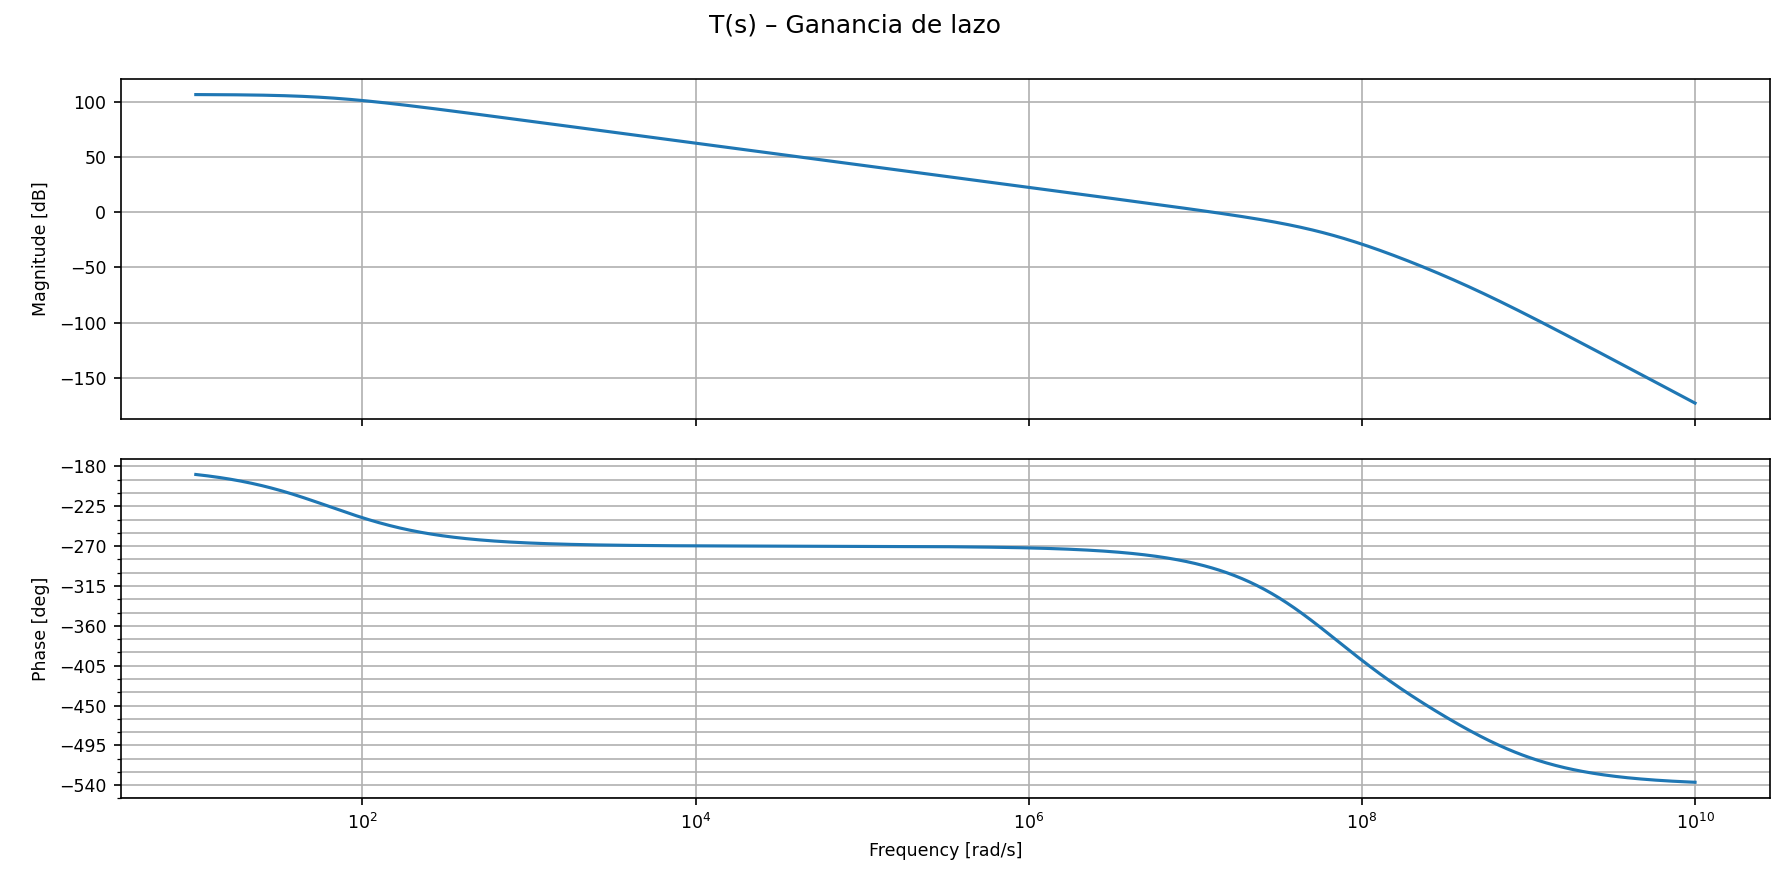
\includegraphics[width=1\linewidth]{T_C3.png}
    \caption{Diagrama de Bode de $T(s)$}
    \label{fig:placeholder}
\end{figure}

\begin{figure}[H]
    \centering
    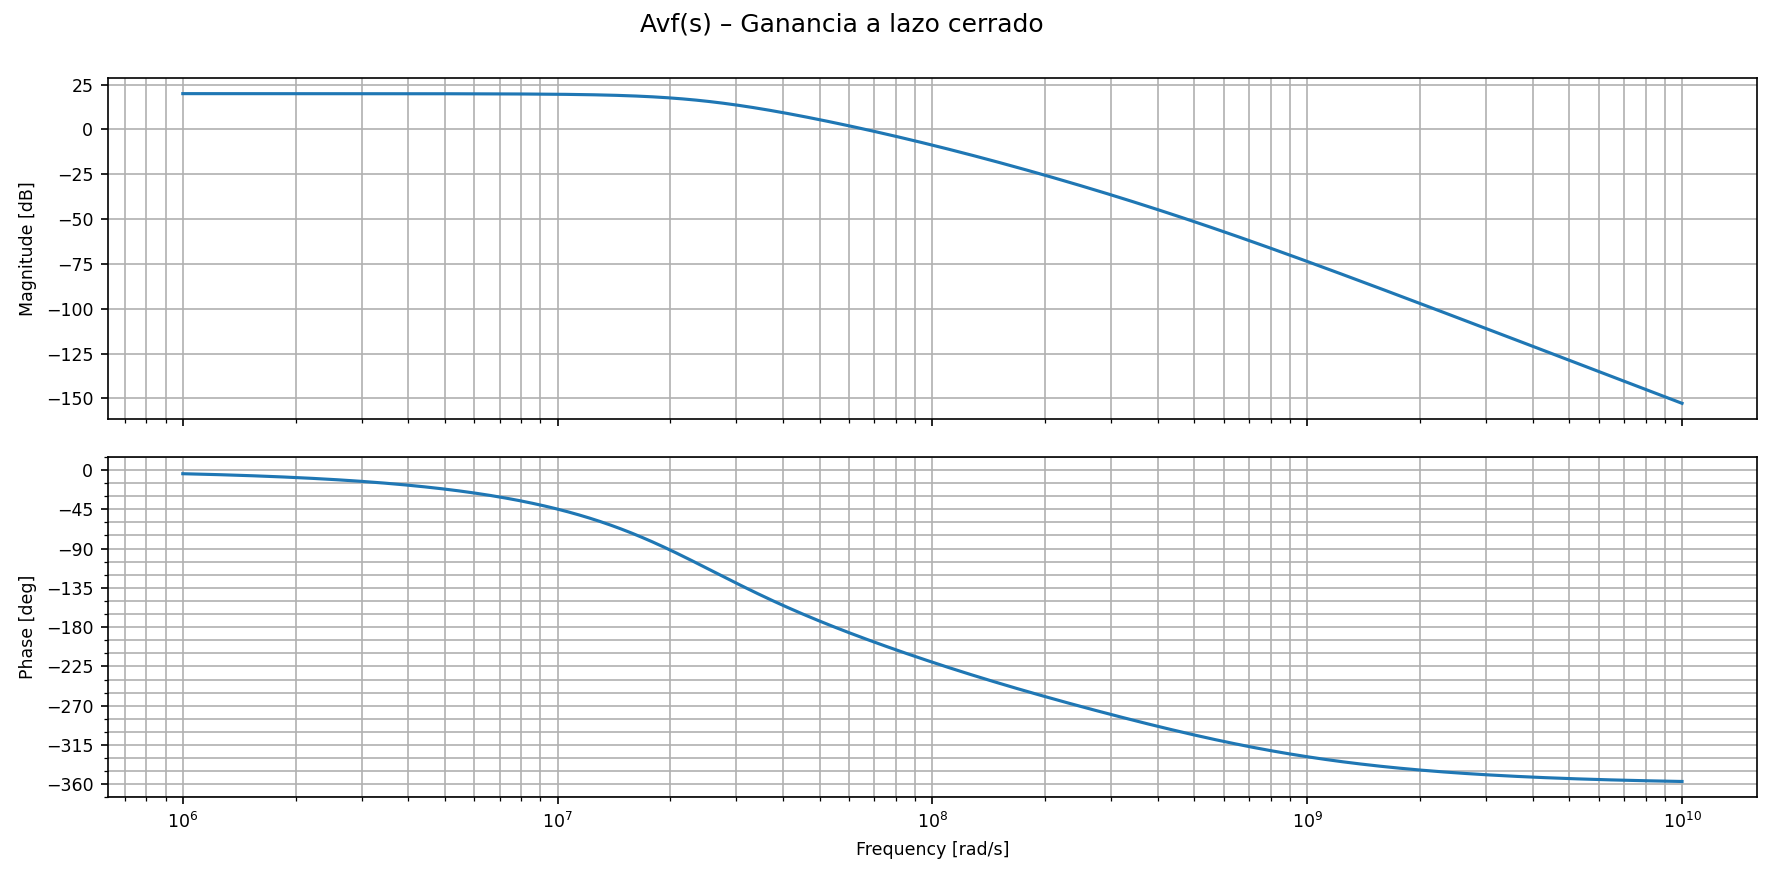
\includegraphics[width=1\linewidth]{Avf_C3.png}
    \caption{Diagrama de Bode de $A_{vf}(s)$}
    \label{fig:placeholder}
\end{figure}

\begin{equation}
\label{eq_116}
M\phi = \ang{65,35}
\end{equation}
\hspace{0.5 cm}

Gracias a los diagramas es posible notar que se alcanza correctamente el valor de ganancia global requerido, como así también el Margen de Fase, además del $f_G$ para el cual se calcularon las resistencias, ya que puede observarse $\omega_G = 1,25\,.\,10^7[\frac{rad}{s}]$. El diagrama de Bode también muestra que la caída de $-3~[dB]$ del sistema se encuentra en:

\begin{equation}
\label{eq_117}
f_p = 3,46~[MHz]
\end{equation}
\hspace{0.5 cm}

El mismo código también grafica la respuesta al escalón del sistema, y los valores del Nivel Máximo $y_{max}$, el Sobrepasamiento $M_p$, el Factor de Amortiguación $\zeta$ y el Margen de Fase estimado, utilizando las ecuaciones expresadas anteriormente en (\ref{eq_80}), (\ref{eq_81}) y (\ref{eq_82}):

\begin{figure}[H]
    \centering
    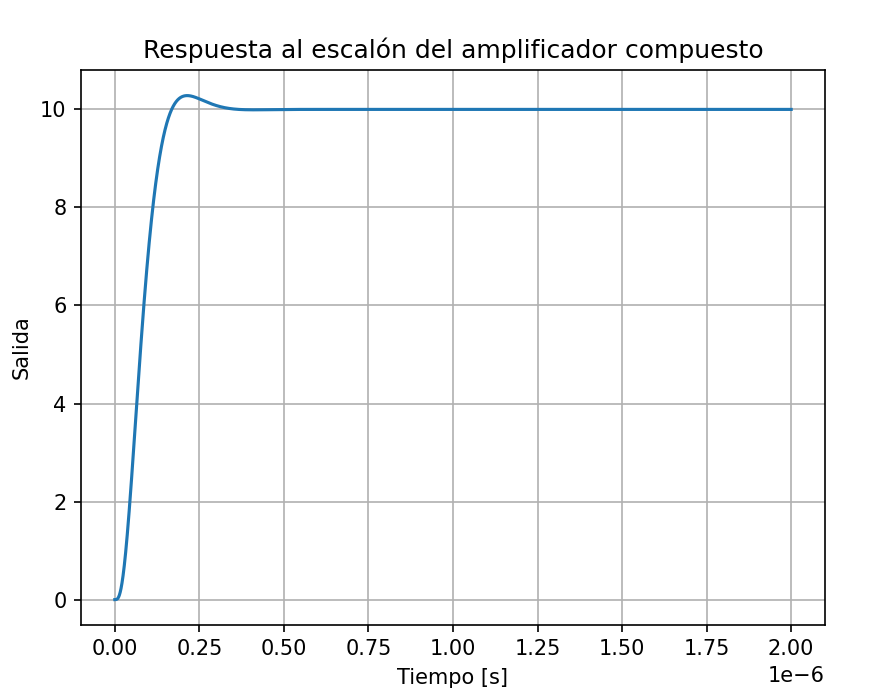
\includegraphics[width=0.7\linewidth]{Step_C3.png}
    \caption{Respuesta al escalón del circuito III}
    \label{fig:placeholder}
\end{figure}

\begin{equation}
\label{eq_118}
y_{max} =  10,282
\end{equation}

\begin{equation}
\label{eq_119}
M_p =  2,82~\%
\end{equation}

\begin{equation}
\label{eq_120}
\zeta =  0,751
\end{equation}

\begin{equation}
\label{eq_121}
M\phi =  \ang{67,68}
\end{equation}
\hspace{0.5 cm}

\subsection{Conclusión parcial:}

Se cumplen los requerimientos establecidos por el objetivo verificando los mismos de distintas formas.

Si bien la incorporación de la red cero–polo en el Circuito III modifica la dinámica interna del sistema, cancelando explícitamente el polo más alejado del $VFA$ y aportando fase positiva alrededor de la frecuencia crítica, como consecuencia, el sistema presenta inicialmente un Margen de Fase superior al requerido, evidenciando una mejora en términos de estabilidad relativa y amortiguación.

El posterior reajuste del $CFA$ permite recuperar el Margen de Fase especificado sin alterar la ganancia global, logrando un diseño donde la compensación se reparte entre etapas en lugar de recaer exclusivamente sobre el amplificador $CFA$.

Por lo tanto, si bien ambos enfoques conducen a resultados similares en cuanto a desempeño final, el uso de la red cero–polo ofrece una mayor flexibilidad de diseño y un mejor control de la relación entre estabilidad y velocidad.
\\

\subsection{Simulación:}

Se dispuso el siguiente circuito en LTspice tal que se analice su comportamiento y similitud con lo calculado teóricamente. Los modelos utilizados para los amplificadores son los mismos que el circuito anterior, se encuentran en el Anexo (\ref{modelo_VFA}) y (\ref{modelo_CFA}):

\begin{figure}[H]
    \centering
    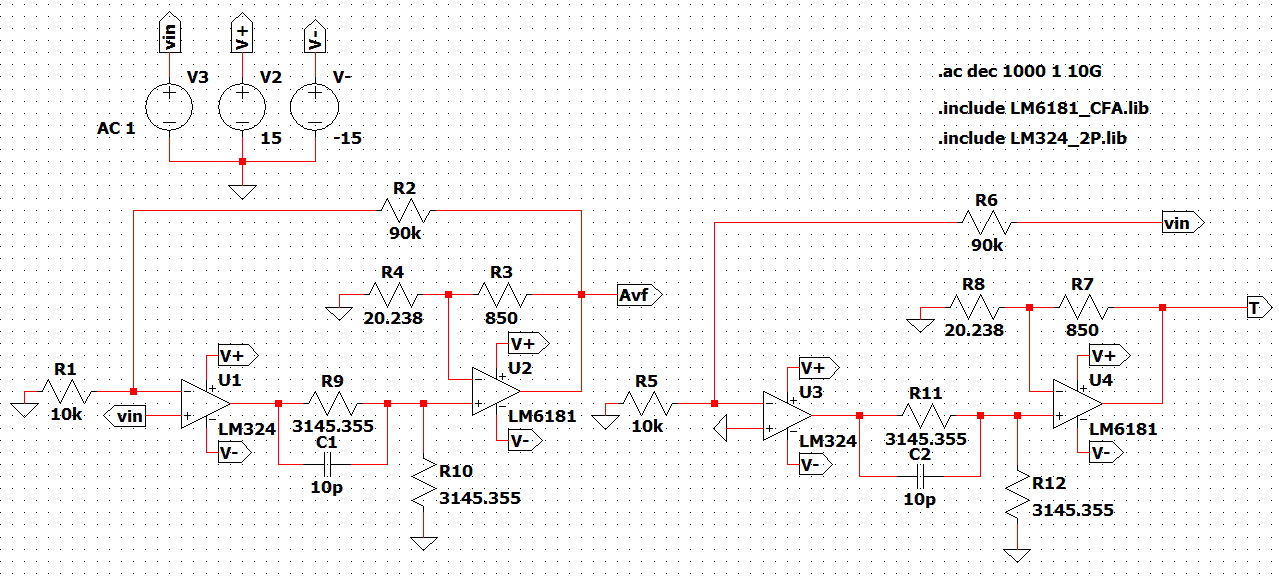
\includegraphics[width=1\linewidth]{Spice_C3.png}
    \caption{Diagrama circuital en LTspice}
    \label{fig:placeholder}
\end{figure}

Con este circuito pudieron graficarse los diagramas de bode de $A_{vf}(s)$ y $T(s)$ para ambos casos de la sección, primero se presentan los resultados para antes del ajuste de $R_2$ y $R_1$:

\begin{figure}[H]
    \centering
    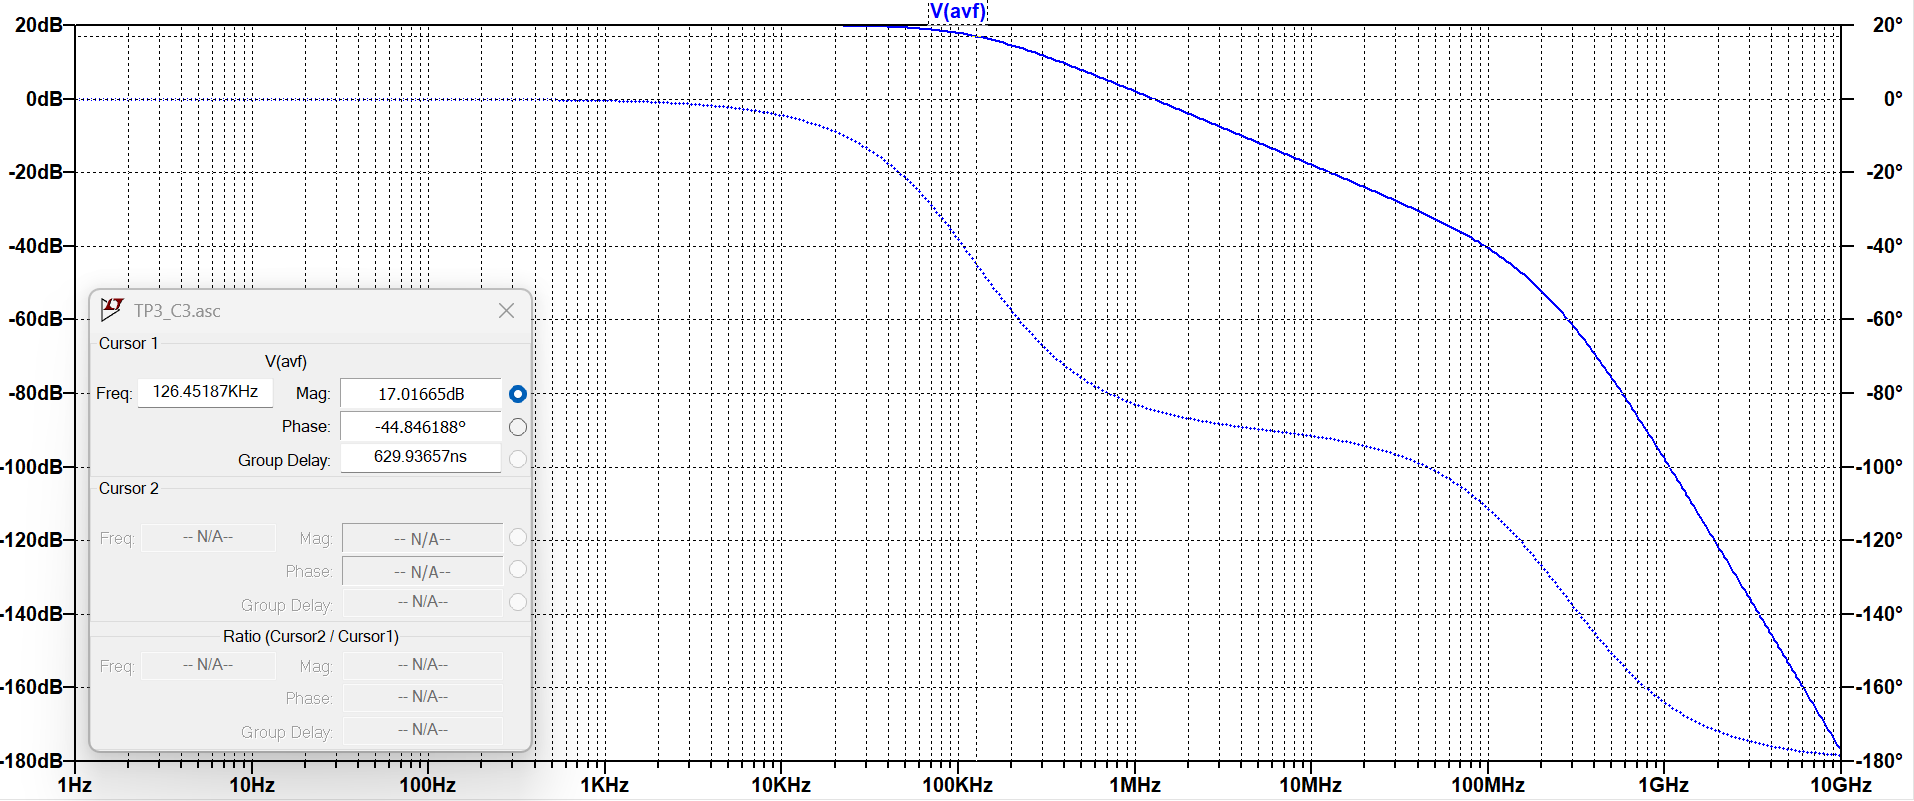
\includegraphics[width=1\linewidth]{Bode_Avf_Spice_C3_Amort.png}
    \caption{Diagrama de Bode de $A_{vf}(s)$}
    \label{fig:placeholder}
\end{figure}

En este puede verse que se alcanza el valor de ganancia global presentado en el objetivo del circuito, sin embargo esta cae más temprano que lo calculado, esta vez en $f_p = 126~[kHz]$. 
\\

\begin{figure}[H]
    \centering
    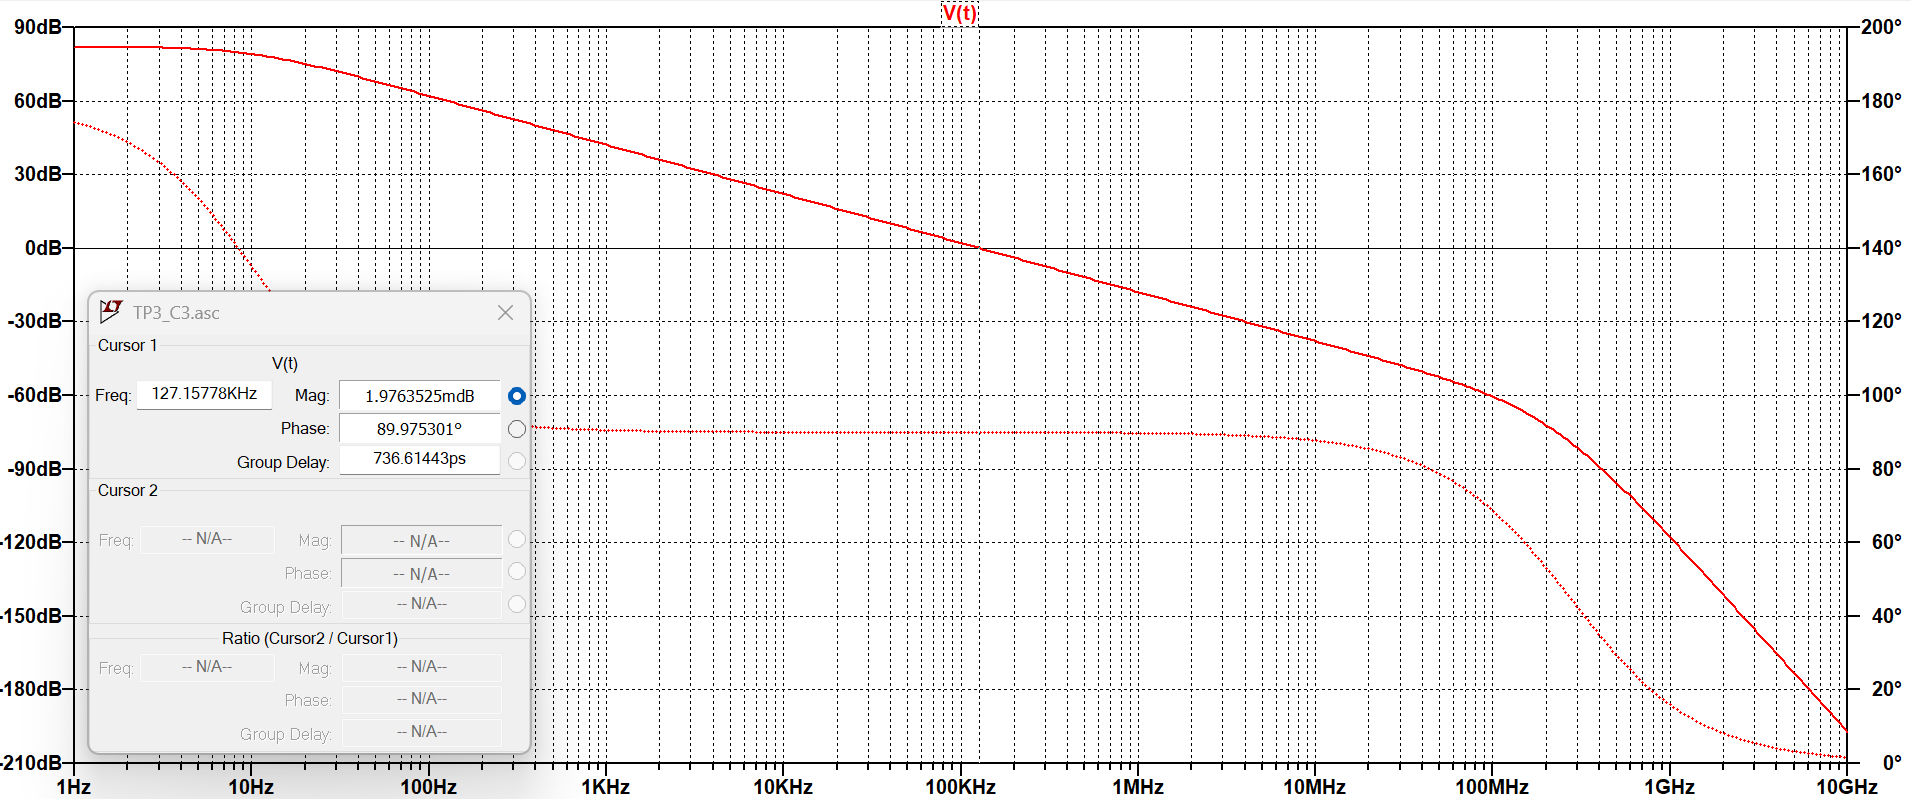
\includegraphics[width=1\linewidth]{Bode_T_Spice_C3_Amort.png}
    \caption{Diagrama de Bode de $T(s)$}
    \label{fig:placeholder}
\end{figure}

El cursor en este caso marca el valor de $\left|T(s)\right|=0~[dB]$ en la frecuencia que corresponde al punto crítico y logra verse $f_G=126~[kHz]$. También se aprecia en ese punto una fase de $\phi=\ang{90}$.

Semejante al caso de este circuito antes del ajuste de las resistencias, puede mencionarse una mejora del Margen de Fase en términos de estabilidad. Sin embargo, la simulación del programa muestra una caída del ancho de banda que el código de Python no demostró anteriormente.
\\

\subsubsection{Ajuste de $R_2$ y $R_1$:}

De la misma forma que en el cálculo teórico, se busca mejorar el Margen de Fase para lograr la Máxima Planicidad de Módulo, para esto se ajustan las resistencias en el LTspice a las calculadas en las ecuaciones (\ref{eq_114}) y (\ref{eq_115}).

A partir de esto se graficaron los diagramas de $A_{vf}(s)$ y $T(s)$ y se muestran a continuación:

\begin{figure}[H]
    \centering
    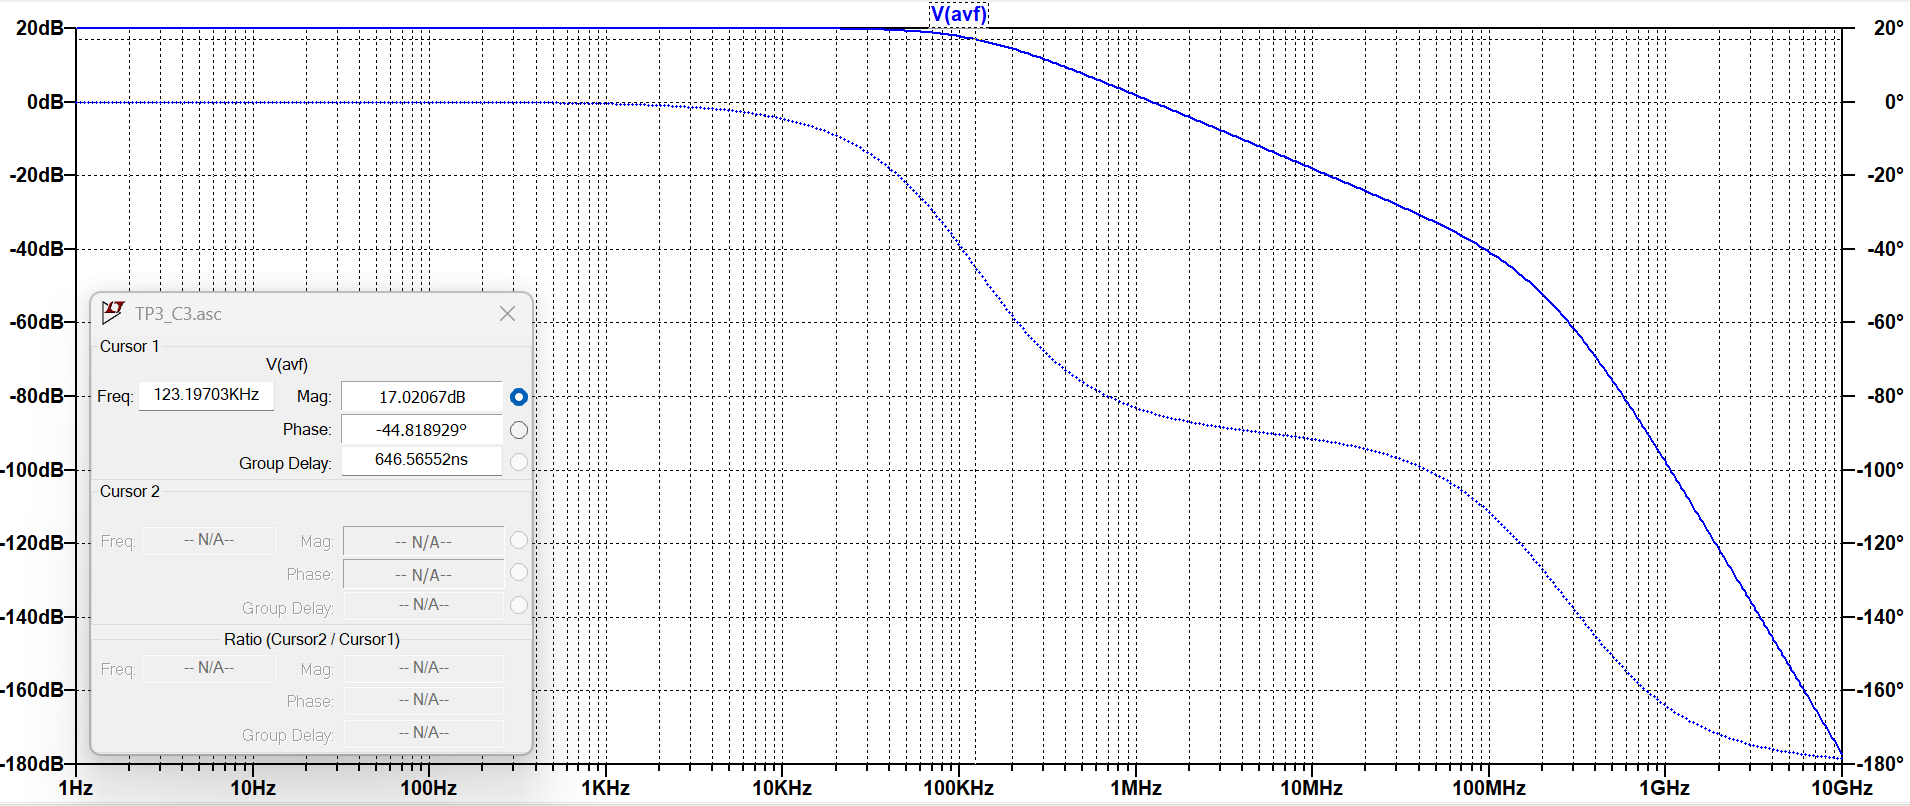
\includegraphics[width=1\linewidth]{Bode_Avf_Spice_C3.png}
    \caption{Diagrama de Bode de $A_{vf}(s)$}
    \label{fig:placeholder}
\end{figure}

\begin{figure}[H]
    \centering
    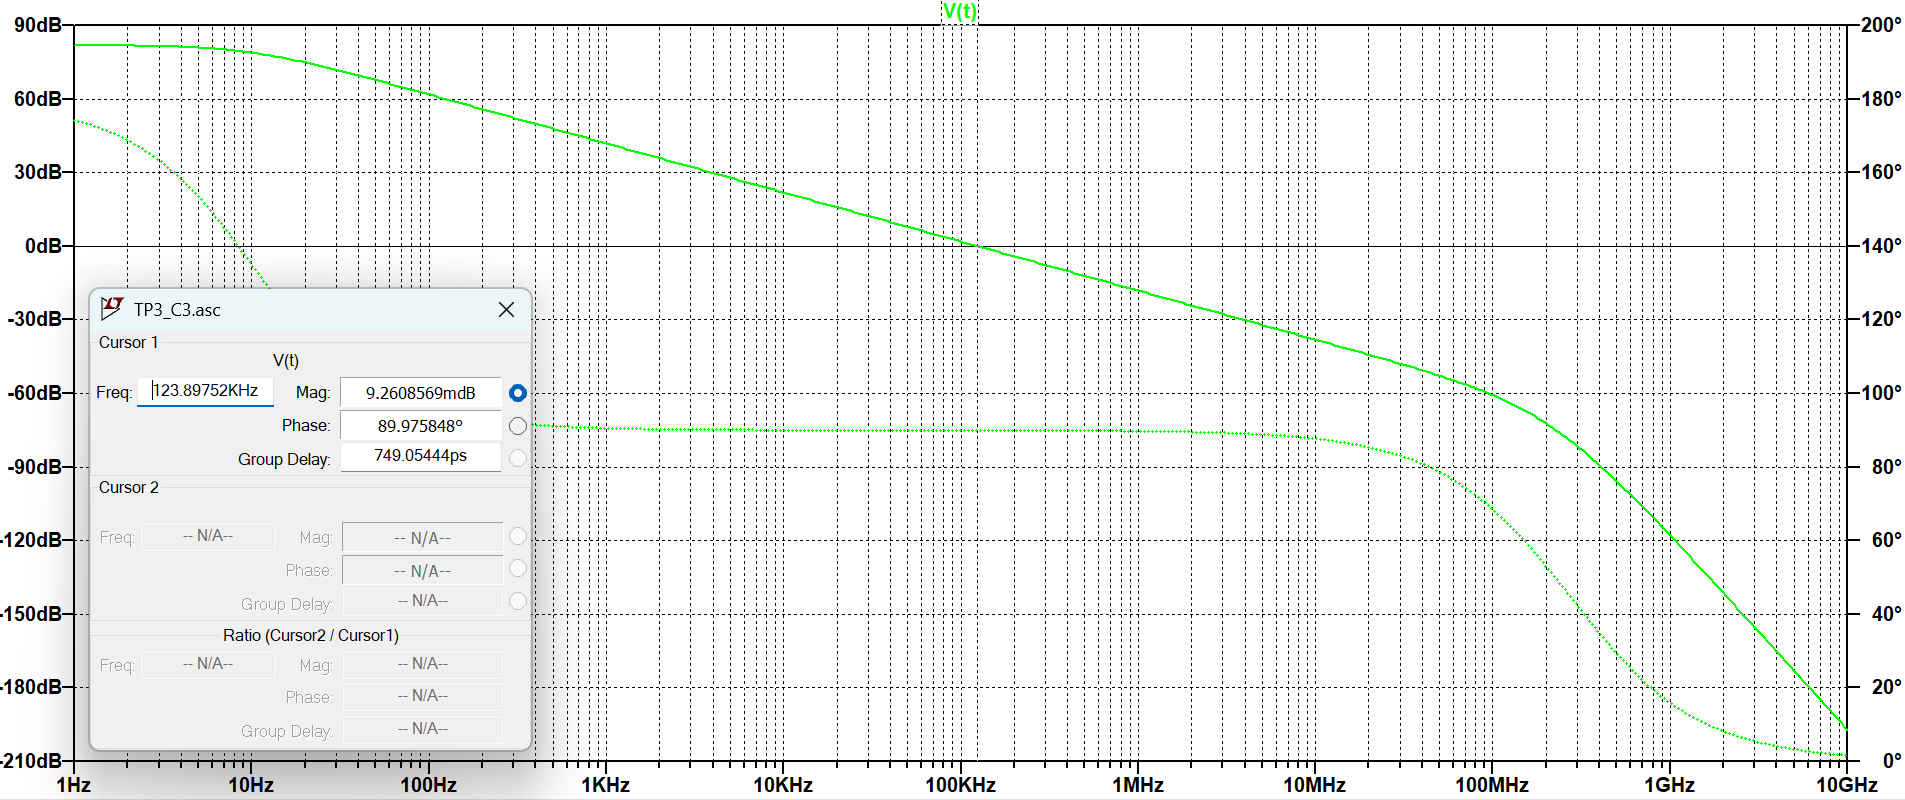
\includegraphics[width=1\linewidth]{Bode_T_Spice_C3.png}
    \caption{Diagrama de Bode de $T(s)$}
    \label{fig:placeholder}
\end{figure}

Es posible ver que en ambos casos el ajuste de resistencias produjo cambios mínimos en el sistema, ya que el Margen de Fase sigue siendo $M\phi = \ang{90}$ y la frecuencia de punto crítico, que cae en el mismo lugar que el punto de caída de$-3~[dB]$, se encuentra en $f_p = f_G = 123~[kHz]$. Sin embargo, la ganancia global sí se logró en ambos casos.

\newpage
\section{Conclusiones}

En el presente trabajo se analizó y diseñó un amplificador compuesto con el objetivo de cumplir simultáneamente con una ganancia a lazo cerrado de $20~[dB]$ y un Margen de Fase especificado.

A partir del modelado en pequeña señal de ambos amplificadores mediante funciones de transferencia de segundo orden, se construyó la ganancia de lazo del sistema completo, la cual resulta de cuarto orden debido a la combinación de los polos propios del $VFA$ y de la dinámica introducida por la realimentación local del $CFA$ en cada caso.

En cuanto a los resultados, el circuito I no pudo lograr simultáneamente ambos requerimientos, mientras que de los dos siguientes circuitos, el circuito II se comportó correctamente por todas las verificaciones posibles, y el circuito III si bien los cálculos teóricos dieron resultados coherentes, la simulación en el LTspice no coincidió con los anteriores.

El trabajo pone en evidencia la importancia del análisis en frecuencia como herramienta principal para la evaluación de estabilidad en sistemas de control analógicos.


\newpage
\appendix
\section{Códigos del proyecto}

\subsection{Circuito I:}

\lstinputlisting[language=python, caption={Obtención de polos de FT.}, label={codigo1}]{Get_Poles.Py}
\hspace{0.5 cm}

\lstinputlisting[language=python, caption={Gráfico de $A_{vf}(s)$ simple.}, label={codigo2}]{Plot_Avf_Simple.Py}
\hspace{0.5 cm}

\lstinputlisting[language=python, caption={Barrido Margen de Fase vs. $k=\frac{R_2}{R_1}$.}, label={codigo3}]{k_vs_MF.Py}
\hspace{0.5 cm}

\lstinputlisting[language=python, caption={Margen de Fase para $k=\frac{R_2}{R_1}<0$.}, label={codigo4}]{Circuito1_R_Negativa.Py}
\hspace{0.5 cm}

\subsection{Circuito II:}

\lstinputlisting[language=python, caption={Barrido de $R_1$ para $f_G$.}, label={codigo5}]{Barrido_R1_C2.py}
\hspace{0.5 cm}

\lstinputlisting[language=python, caption={Verificación de valores.}, label={codigo6}]{Verificacion_C2.py}
\hspace{0.5 cm}

\lstinputlisting[language=python, caption={Respuesta al escalón.}, label={codigo7}]{Step_C2.py}
\hspace{0.5 cm}

\lstinputlisting[language=python, caption={Obtención de polos de FT.}, label={codigo8}]{Get_Poles_C2.py}
\hspace{0.5 cm}

\subsection{Circuito III:}

\lstinputlisting[language=python, caption={Análisis de la red cero-polo.}, label={codigo9}]{Red_RC_C3.py}
\hspace{0.5 cm}

\lstinputlisting[language=python, caption={Análisis del sistema total.}, label={codigo10}]{Get_Poles_C3.py}
\hspace{0.5 cm}

\lstinputlisting[language=python, caption={Respuesta al escalón del sistema amortiguado.}, label={codigo11}]{Step1_C3.py}
\hspace{0.5 cm}

\lstinputlisting[language=python, caption={Barrido de $R_1$ para $f_G$.}, label={codigo12}]{Barrido_R1_C3.py}
\hspace{0.5 cm}

\lstinputlisting[language=python, caption={Verificación de valores.}, label={codigo13}]{Verificacion_C3.py}
\hspace{0.5 cm}

\subsection{Modelos de SPICE:}

\lstinputlisting[language=python, caption={Modelo de LM324 para LTspice}, label={modelo_VFA}]{LM324_2P.lib}
\hspace{0.5 cm}

\lstinputlisting[language=python, caption={Modelo de LM6181 para LTspice}, label={modelo_CFA}]{LM6181_CFA.lib}
\hspace{0.5 cm}

\end{document}